\section{Introduction}

An overview of a search for Supersymmetry in the all-hadronic channel with missing transverse momentum and a customized top tagger is presented. The data used for the analysis was collected in 2016 by the CMS experiment at the LHC, and corresponds to an integrated luminosity of 35.9 fb$^{-1}$ from proton-proton collisions at a center-of-mass energy ($\sqrt{s}$) of 13 TeV. The results and procedures presented are the product of an analysis conducted in collaboration with the hadronic SUSY analysis team based at Fermilab in Batavia, IL, USA. The published results can be obtained from \cite{SUSYanalysis}.

\section{Analysis Description}

The study consists of an inclusive search for events with final states that contain missing transverse momentum ($p_{\text{T}}^{miss}$) and reconstructed top quarks. The signal models used in this study include the production of three different types of SUSY particles. Two of which are the top squark ($\tilde{t}$) and the gluino ($\tilde{g}$), the supersymmetric partners of the SM top quark (t) and gluon (g). The third one is the neutralino ($\tilde{\chi}_{1}^{0}$), considered to be the lightest SUSY particle (LSP) under the Minimal Supersymmetric Standard Model (MSSM), and a possible candidate for Dark Matter.\\

The signal data is selected by requiring events to have a minimum amount of jets ($N_\text{j}$) and b-jets ($N_\text{b}$) as well as a large $p_{\text{T}}^{miss}$. Other factors, such as the number of top jets ($N_\text{t}$), the scalar sum of the jet transverse momentum ($H_\text{T}$), and the so-called stransverse mass ($m_\text{T2}$)\footnote{$m_\text{T2}$ is a minimization of two transverse masses ($m_\text{T}$) with a constraint that the sum of the transverse momenta of both $\tilde{\chi}_{1}^{0}$'s is equal to the transverse momentum of the event, i.e., $\vec{p}_\text{T} = \vec{q}_\text{T}^{(1)} + \vec{q}_\text{T}^{(2)}$. The mathematical definition is given by $m_\text{T2} \equiv \underset{\vec{q}_\text{T}^{(1)} + \vec{q}_\text{T}^{(2)} = \vec{p}_\text{T}}{\text{min}}\left [ \text{max}\left \{ m_\text{T}^2 (\vec{p}_\text{T}^{(1)}, \vec{q}_\text{T}^{(1)}; m_{\tilde{\chi}_{1}^{0}}), (\vec{p}_\text{T}^{(2)}, \vec{q}_\text{T}^{(2)}; m_{\tilde{\chi}_{1}^{0}}) \right \} \right ]$.} are also considered in order to select events of interest. The search region is then defined in exclusive bins of $N_\text{t}$, $N_\text{b}$, $H_\text{T}$, $p_{\text{T}}^{miss}$ and $m_\text{T2}$. Additional discriminatory variables used in the analysis include the azimuthal angle between $p_{\text{T}}^{miss}$ and the leading jets of an event ($\Delta\phi$), the pseudorapidity ($\eta$) and the cone radius size (defined as $\Delta R = \sqrt{(\Delta\eta)^2+(\Delta\phi)^2}$) used in the isolation of various physics objects.

\subsection{Signal Models}

The signal models used in this analysis are based on two different scenarios: direct top squark production and gluino mediated top squark production. In the former scenario we consider one decay within the Simplified Model Spectra (SMS)\cite{SMS} framework called `T2tt' (\autoref{SignalModels.png}, top left), where a top squark pair is produced directly from the proton-proton collision and then decays into a pair of top quarks and a pair of neutralinos ($\tilde{\text{t}}\rightarrow\text{t}\tilde{\chi}_{1}^{0}$).\\

\begin{figure}[H]
\begin{center}
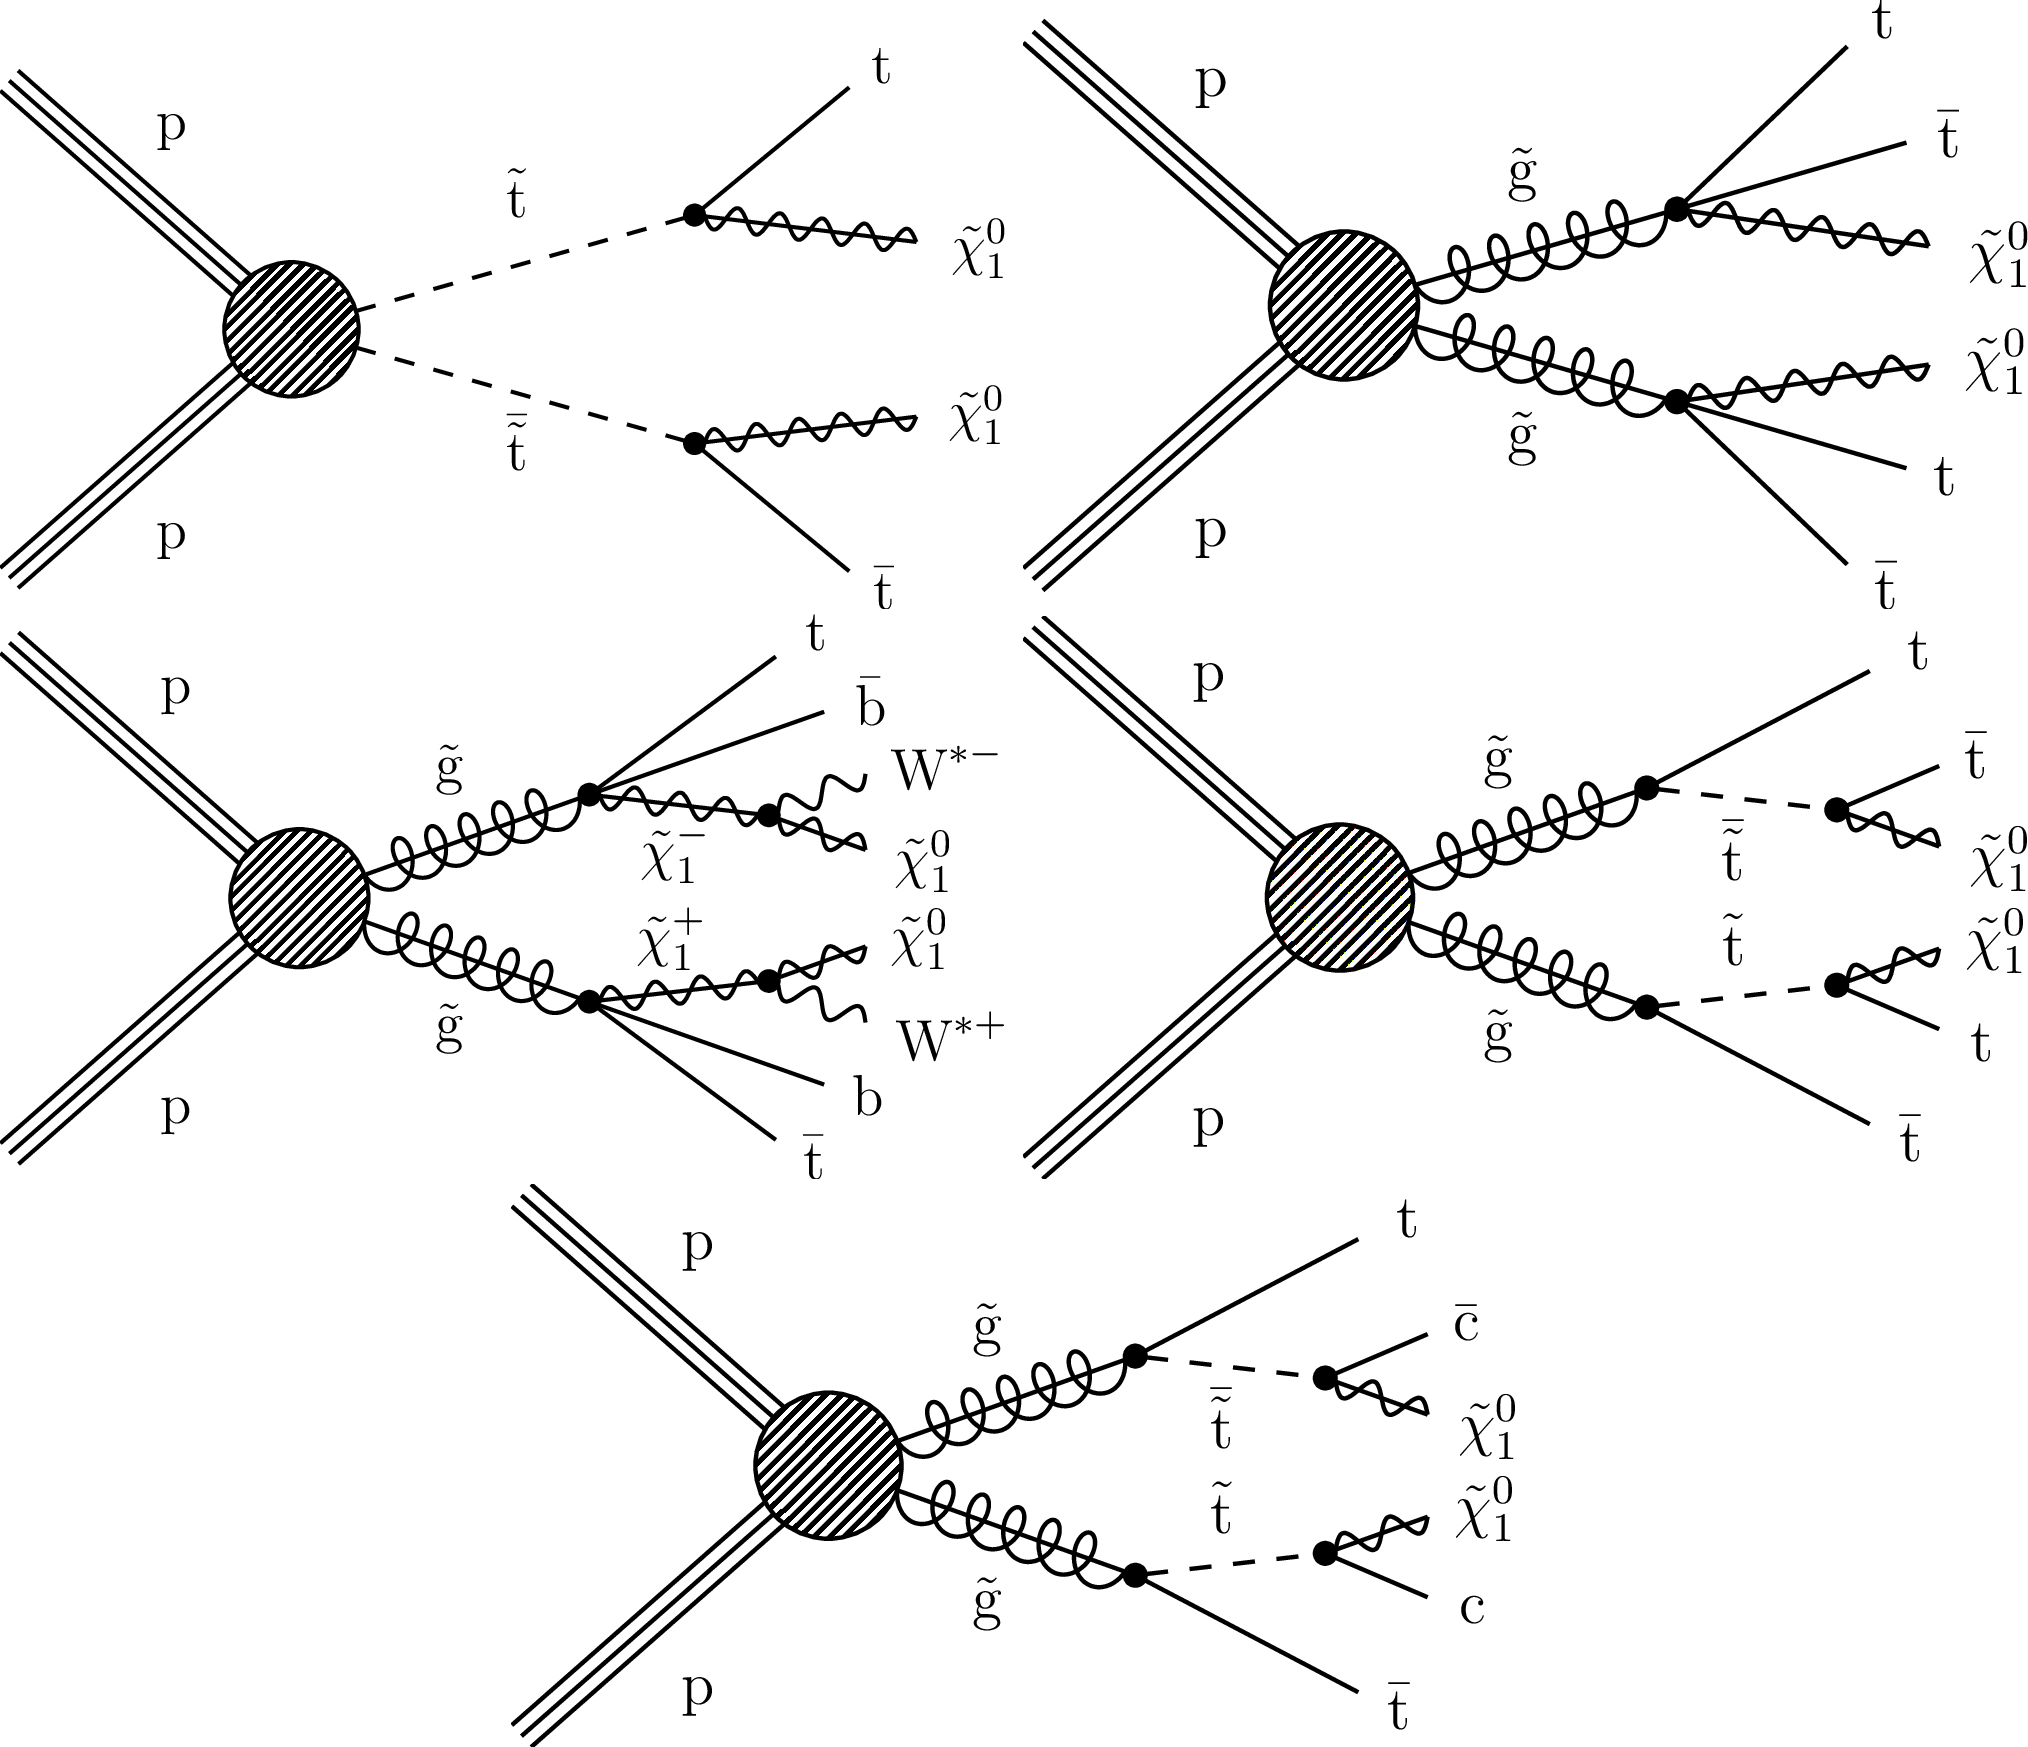
\includegraphics[width=0.92\textwidth]{SignalModels.png} 
\caption{Simplified model diagrams show of the various Supersymmetry signals considered in this analysis: the T2tt model (top left), the T1tttt model (top right), the T1ttbb model (middle left), the T5tttt (middle right), and the T5ttcc model (bottom).}
\label{SignalModels.png} 
%\hspace{4em}
\end{center}
\end{figure}

In the case of gluino mediated top squark production there are several different decay modes considered. The T1tttt model (\autoref{SignalModels.png}, top right) consists of two gluinos decaying into a pair of top quarks and a neutralino ($\tilde{\text{g}}\rightarrow\text{t}\bar{\text{t}}\tilde{\chi}_{1}^{0}$), accounting for situations in which the top squark is too heavy to be produced directly but the gluino is not. In the T1ttbb model (\autoref{SignalModels.png}, middle left), a pair of gluinos to either a top or bottom squark as $\tilde{\text{g}}\rightarrow\text{t}\bar{\text{t}}\tilde{\chi}_{1}^{0}$ (25\%), $\tilde{\text{g}}\rightarrow\text{b}\bar{\text{b}}\tilde{\chi}_{1}^{0}$ (25\%), or $\tilde{\text{g}}\rightarrow\bar{\text{t}}\text{b}\tilde{\chi}_{1}^{\pm}$ (50\%), where $\tilde{\chi}_{1}^{\pm}$ denotes the lightest positive ($\tilde{\chi}_{1}^{+}$) or negative ($\tilde{\chi}_{1}^{-}$) chargino. Due to the small difference in mass between the $\tilde{\chi}_{1}^{+}$ (or its conjugate) and the LSP ($\Delta m(\tilde{\chi}_{1}^{+},\tilde{\chi}_{1}^{0}) = 5$ GeV), the two particles are taken to be nearly mass degenerate. The T1ttbb model provides sensitivity to situations where there are mixed states of top and bottom squarks.\\

The T5tttt model consists of a pair of gluinos, where each decays into a top quark and an on-shell top squark. The top squark then decays into a top quark and a neutralino. For this model, a mass difference of $\Delta m(\tilde{\text{t}},\tilde{\chi}_{1}^{0}) = 175$ GeV between the top squark and the LSP is expected. This model provides sensitivity to a region of T2tt where the t$\bar{\text{t}}$ background is very similar to the signal and $\Delta m(\tilde{\text{t}},\tilde{\chi}_{1}^{0})$ is very close to the top squark mass. In the T5ttcc model (\autoref{SignalModels.png}, bottom) each gluino decays into a final state consisting of a top quark, a charm quark and a neutralino ($\tilde{\text{g}}\rightarrow\bar{\text{t}}\text{c}\tilde{\chi}_{1}^{0}$). This model is very similar to the T5tttt model with the difference that $\Delta m(\tilde{\text{t}},\tilde{\chi}_{1}^{0}) = 20$ GeV and the on-shell top squark decays into a charm quark and the LSP. The T5ttcc model provides sensitivity to situations where the on-shell top squark is kinematically forbidden from decaying into a top quark.\\

All five signal models described share similar final states containing two neutralinos and up to four top quarks. Since the neutralino is considered stable and only interacts weakly with matter, it cannot be picked up by the detector. Therefore, missing transverse momentum ($p_{T}^{miss}$) is one of the most important variables used to compare event yields between the signal and the SM background.

\subsection{Top Tagger}\label{TopTaggerSec}

The distinguishing feature of this analysis is its powerful top-tagging algorithm. It is designed to provide high reconstruction efficiency over the full range of the top quark $p_\text{T}$ for the considered SUSY signal models. This top-tagger combines the use of several different jet clustering algorithms in order to identify three different categories of top quark jets, designated as ``monojet'', ``dijet'' and ``trijet''. The tagger makes use of identified jets that were reconstructed with the anti-$k_\text{T}$\cite{AntiKt} clustering algorithms combined with additional corrections and selection criteria provided by the Cambridge--Aachen\cite{JetAlg1} and soft-drop de-clustering\cite{SoftDrop} algorithms. In addition, multivariate analysis (MVA) techniques, such as the random forest decision tree algorithm\cite{RandForest1}, were applied in order to further decrease the amount of reconstructed fake tops.\\

There are three top-quark jet categories that take into account that top quark decay products get closer together as the top quark $p_\text{T}$ becomes higher. For specific $p_\text{T}$ values, the decay products of a hadronic process will be reconstructed either as one (``monojet'') or two (``dijet'') jets rather than three (``trijet''). The $p_\text{T}$ values for which this is observed depends on the size of the jets that are being used. In the case of a highly boosted jet, the anti-$k_\text{T}$ algorithm is used within a cone size $\Delta R \sim 0.8$ (called AK8), which captures all decay products of the top quark and is reconstructed as a single jet. This technique requires that the top quark starts with a $p_\text{T}$ of at least 400 GeV to have the decay products fully captured in the 0.8 jet cone. For a $p_\text{T} < 400$ GeV, resolved top-tagging techniques are more efficient, which require three jets independently clustered within a cone size of $\Delta R \sim 0.4$ (AK4). Both types of algorithms are used in order to obtain a high efficiency over a wide range of top quark $p_\text{T}$.

\begin{figure}[H]
\begin{center}
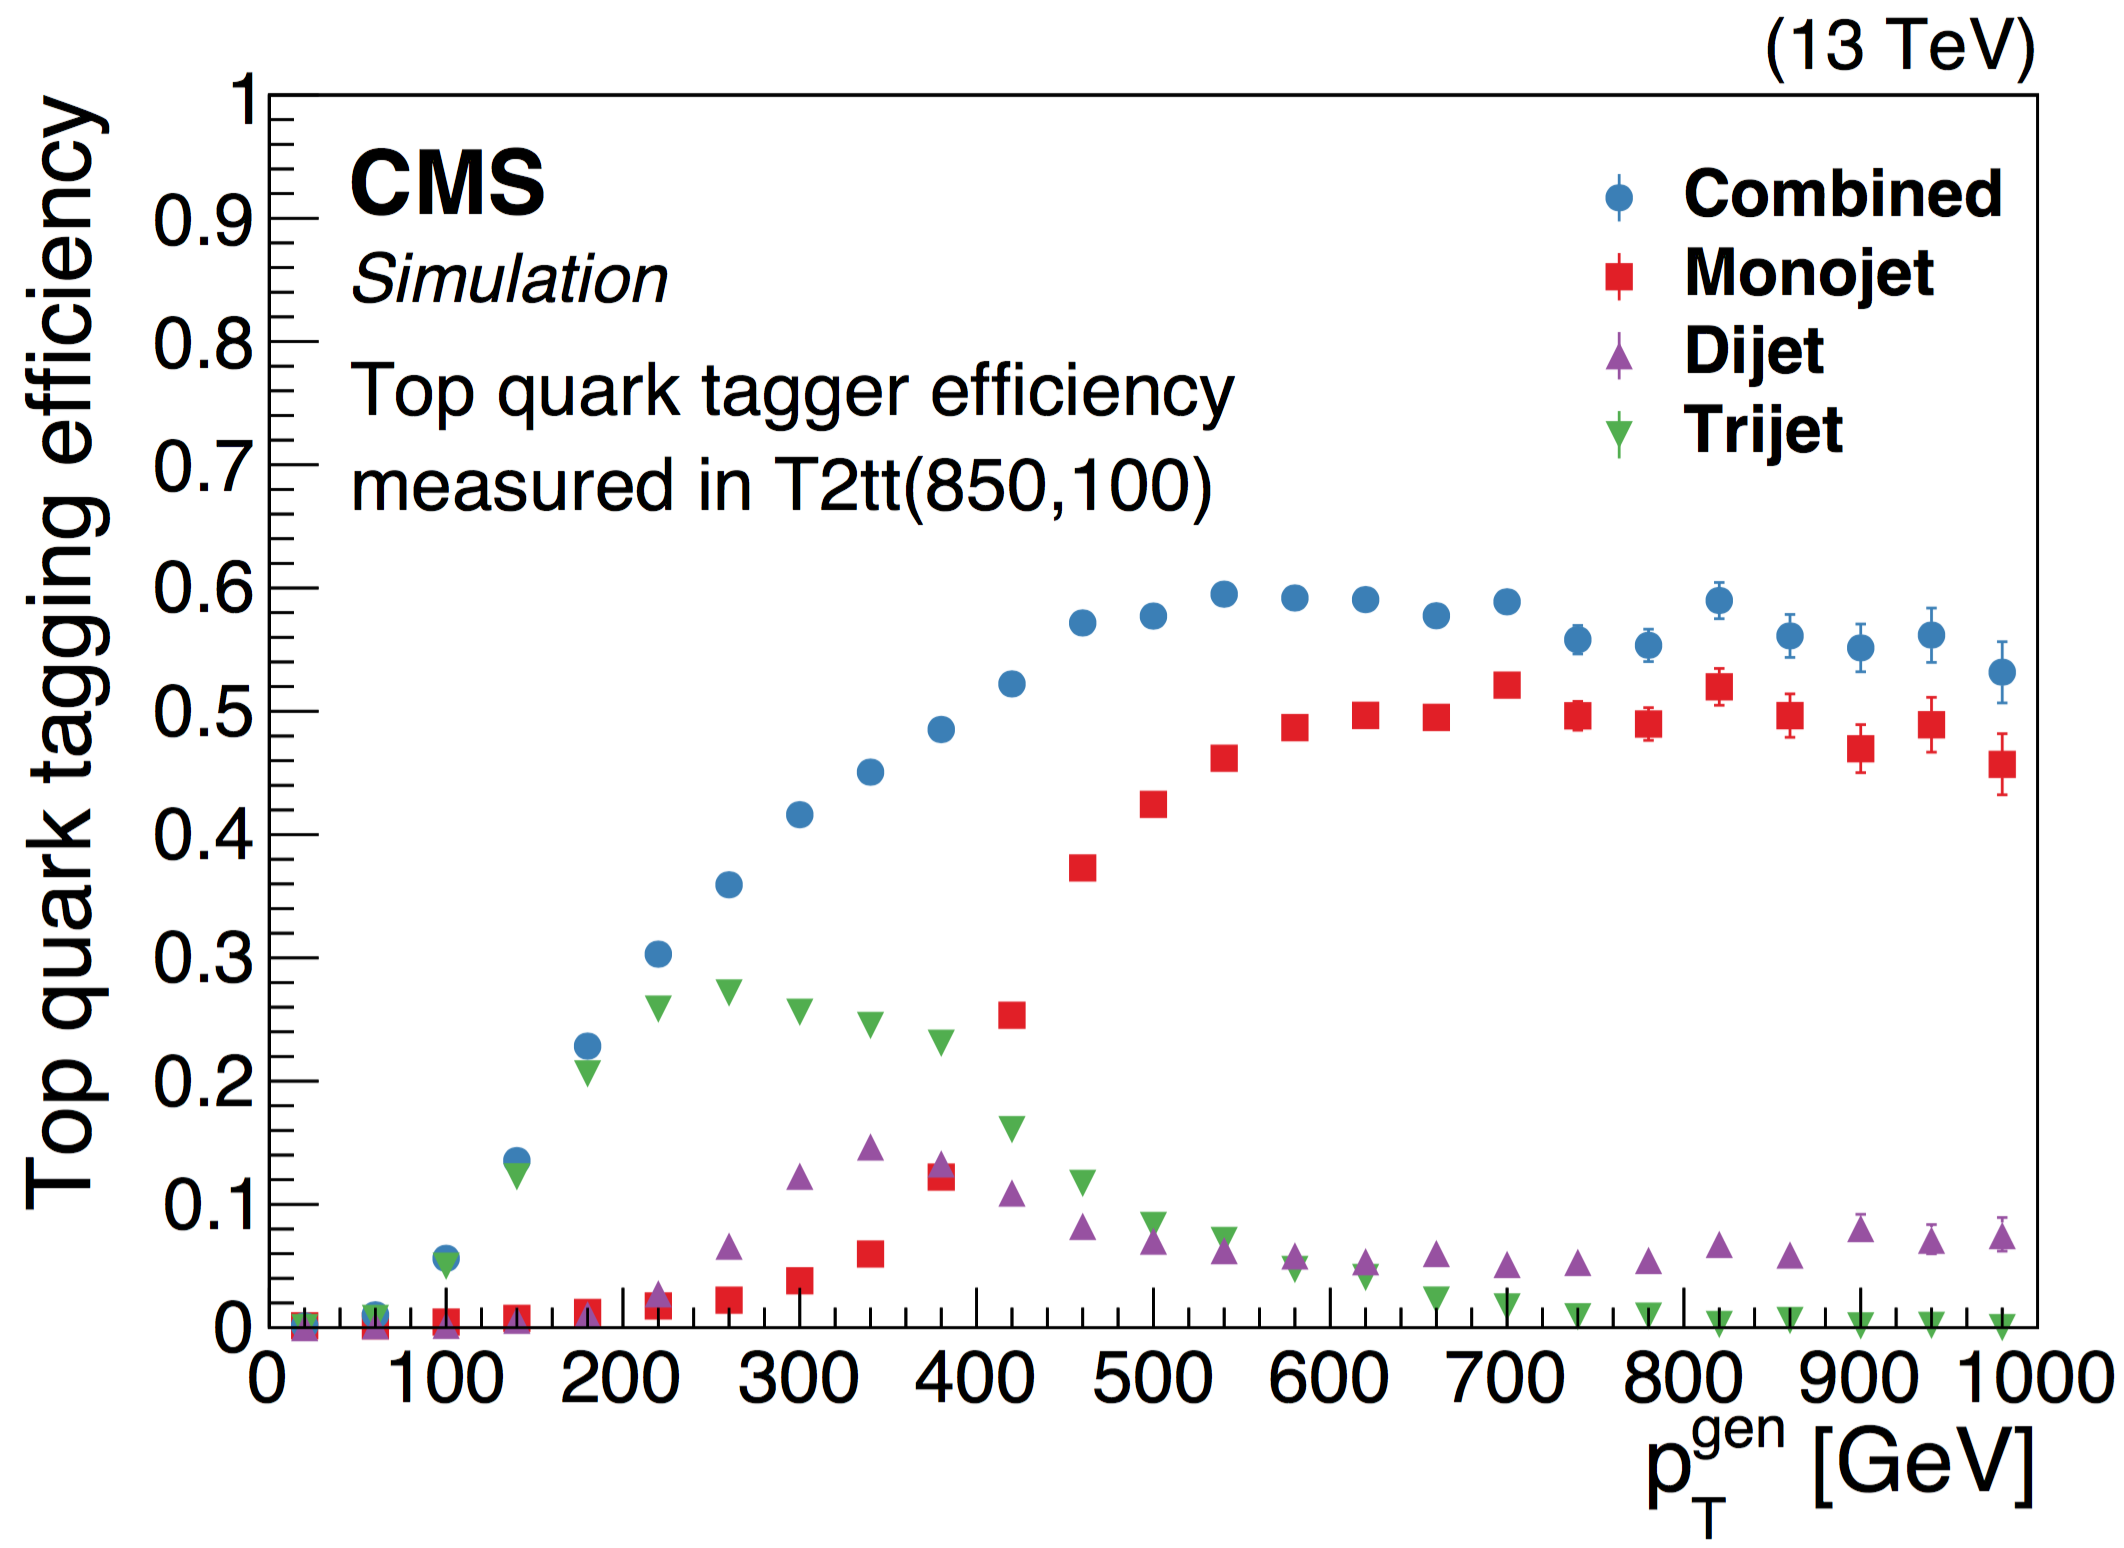
\includegraphics[width=0.8\textwidth]{TopTaggerEff.png} 
\caption{Efficiency of the top quark tagger as a function of generator-level top quark $p_\text{T}$ for the monojet (red boxes), dijet (magenta triangles), and trijet (green upside-down triangles) categories and for their combination (blue circles), as determined using T2tt signal events with a top squark mass of 850 GeV and an LSP mass of 100 GeV. The vertical bars indicate the statistical uncertainties.}
\label{TopTaggerEff} 
\end{center}
\end{figure}

In the case of the dijet top quark decay category, an AK8 jet with a $p_\text{T} > 200$ GeV is combined with a loose AK4 jet to form a top quark candidate. Both jets are required to be within a cone of radius $\Delta R = 1$. For the trijet category, three AK4 jets are combined, with all three jets required to be within a radius of $\Delta R = 1.5$. \autoref{TopTaggerEff} shows the efficiency of the algorithm for each of the three categories of top jets. The efficiency was determined for the T2tt signal model considering a top squark mass of 850 GeV and an LSP mass of 100 GeV, and is calculated as:
\begin{center}
Efficiency $= \dfrac{\text{Number of generator-level top quarks matched to a tagged top}}{\text{Number of generator-level top quarks in an event}}$.
\end{center}

The top quark candidates are required to be within $|\eta| < 2.0$. Furthermore, a cone size of $\Delta R < 0.4$ is used to match the reconstructed top quark to the generated-level top quark. The average misidentification rate as a function of the $p_\text{T}^{miss}$ is found to be around 20\% for simulated Z($\nu\bar{\nu}$)+jets events with a selection criteria similar to the one applied to data: $N_j \geq 4$, $N_b \geq 1$, $p_\text{T}^{miss} > 250$ GeV and no isolated electron or muon with $p_\text{T} > 10$ GeV.


\subsection{Lepton and Track Vetoes}\label{lepVeto}

Since the search only involves models with purely hadronic final states, events which contain electrons or muons are vetoed. This requires the isolation of the muon/electron candidates to a cone size of $\Delta R < 0.2$ for $p_\text{T} \leq 50$ GeV and 0.05 for $\geq 200$ GeV. This $\Delta R$ requirement decreases inversely to the lepton $p_\text{T}$ in the range $50 < p_\text{T} < 200$ GeV in order to account for the collimation of a heavy object's decay products as its Lorentz boost increases. The electron and muon objects are considered to be isolated when their relative isolation\footnote{The ratio between the isolation sum and the candidate $p_\text{T}$.} is less than 0.1 and 0.2, respectively. Due to contributions from pileup, the isolation sum is corrected using an estimate of the amount of pileup energy in the cone.\\

The events that manage to pass the lepton veto are subjected to undergo an isolated charged-particle track veto. The purpose of this veto is to suppress events which contain $\tau$ leptons that decay hadronically or misidentified electrons and muons. The track requirements for this veto are $p_\text{T} > 5$ GeV, $|\eta| < 2.5$ and a relative track isolation less than 0.2. In addition, the isolated track veto is only applied when the transverse mass of an isolated track-$\vec{p}_\text{T}^{miss}$ is $m_\text{T} < 100$ GeV, consistent with W boson decays. This veto successfully reduces the background of leptonically decaying W bosons by about 40\%.

\subsection{Baseline Event Selection}\label{baseline}

The data selection process begins with the triggers and follows with a pre-selection and the definition of the search bins. The selection criteria applied is optimized for high trigger efficiency as well as being sensitive to a variety of new-physics scenarios. The events selected from data meet the following baseline conditions:\\
 
\begin{itemize}
	\item{Satisfy the filters designed to remove detector and beam-related noise.}
	\item{Undergo the lepton, isolated-track, and charged-hadron vetoes.}
	\item{Have a final state with $N_\text{j} \geq 4$, $N_\text{b} \geq 1$, $N_\text{t} \geq 1$, $p_{\text{T}}^{miss} > 250$ GeV and $H_\text{T} > 300$ GeV.}
	\item{$m_\text{T2} > 200$ GeV, in order to reduce background contributions from t$\bar{\text{t}}$ events.}
	\item{To reduce the background arising from the QCD multijet background the azimuthal angle between the $p_{\text{T}}^{miss}$ and the three leading jets of an event is required to be $\Delta\phi(p_{\text{T}}^{miss},j_{1,2,3}) > 0.5, 0.5, 0.3$, where $j_1$, $j_2$, and $j_3$ indicate the three leading jets in order of decreasing $p_\text{T}$.}
\end{itemize}

\subsection{Search Bin Definition}\label{SearchBinDef}

The search described in this chapter was performed by defining 84 non-overlapping search regions (\autoref{SearchBins.png}). Regions that contain events with $N_\text{b} \leq 2$ and $N_\text{t} \leq 2$ use  $N_\text{b}$, $N_\text{t}$, $p_{\text{T}}^{miss}$ and $m_\text{T2}$. In contrast, if the events contain $N_\text{b} \geq 3$ and $N_\text{t} \geq 3$, then $N_\text{b}$, $N_\text{t}$, $p_{\text{T}}^{miss}$ and $H_\text{T}$ are used for that region. The reason $H_\text{T}$ is used for these regions instead of $m_\text{T2}$ has to do with the fact that for events that contain many jets, the jets arising from the decay of specially heavy objects are not always correctly associated with said object, giving the $m_\text{T2}$ variable a relatively broad and flat distribution. Therefore, in regions with $N_\text{b} \geq 3$ and $N_\text{t} \geq 3$, $H_\text{T}$ is found to provide better discrimination between signal and background.

\begin{figure}[tb]
\begin{center}
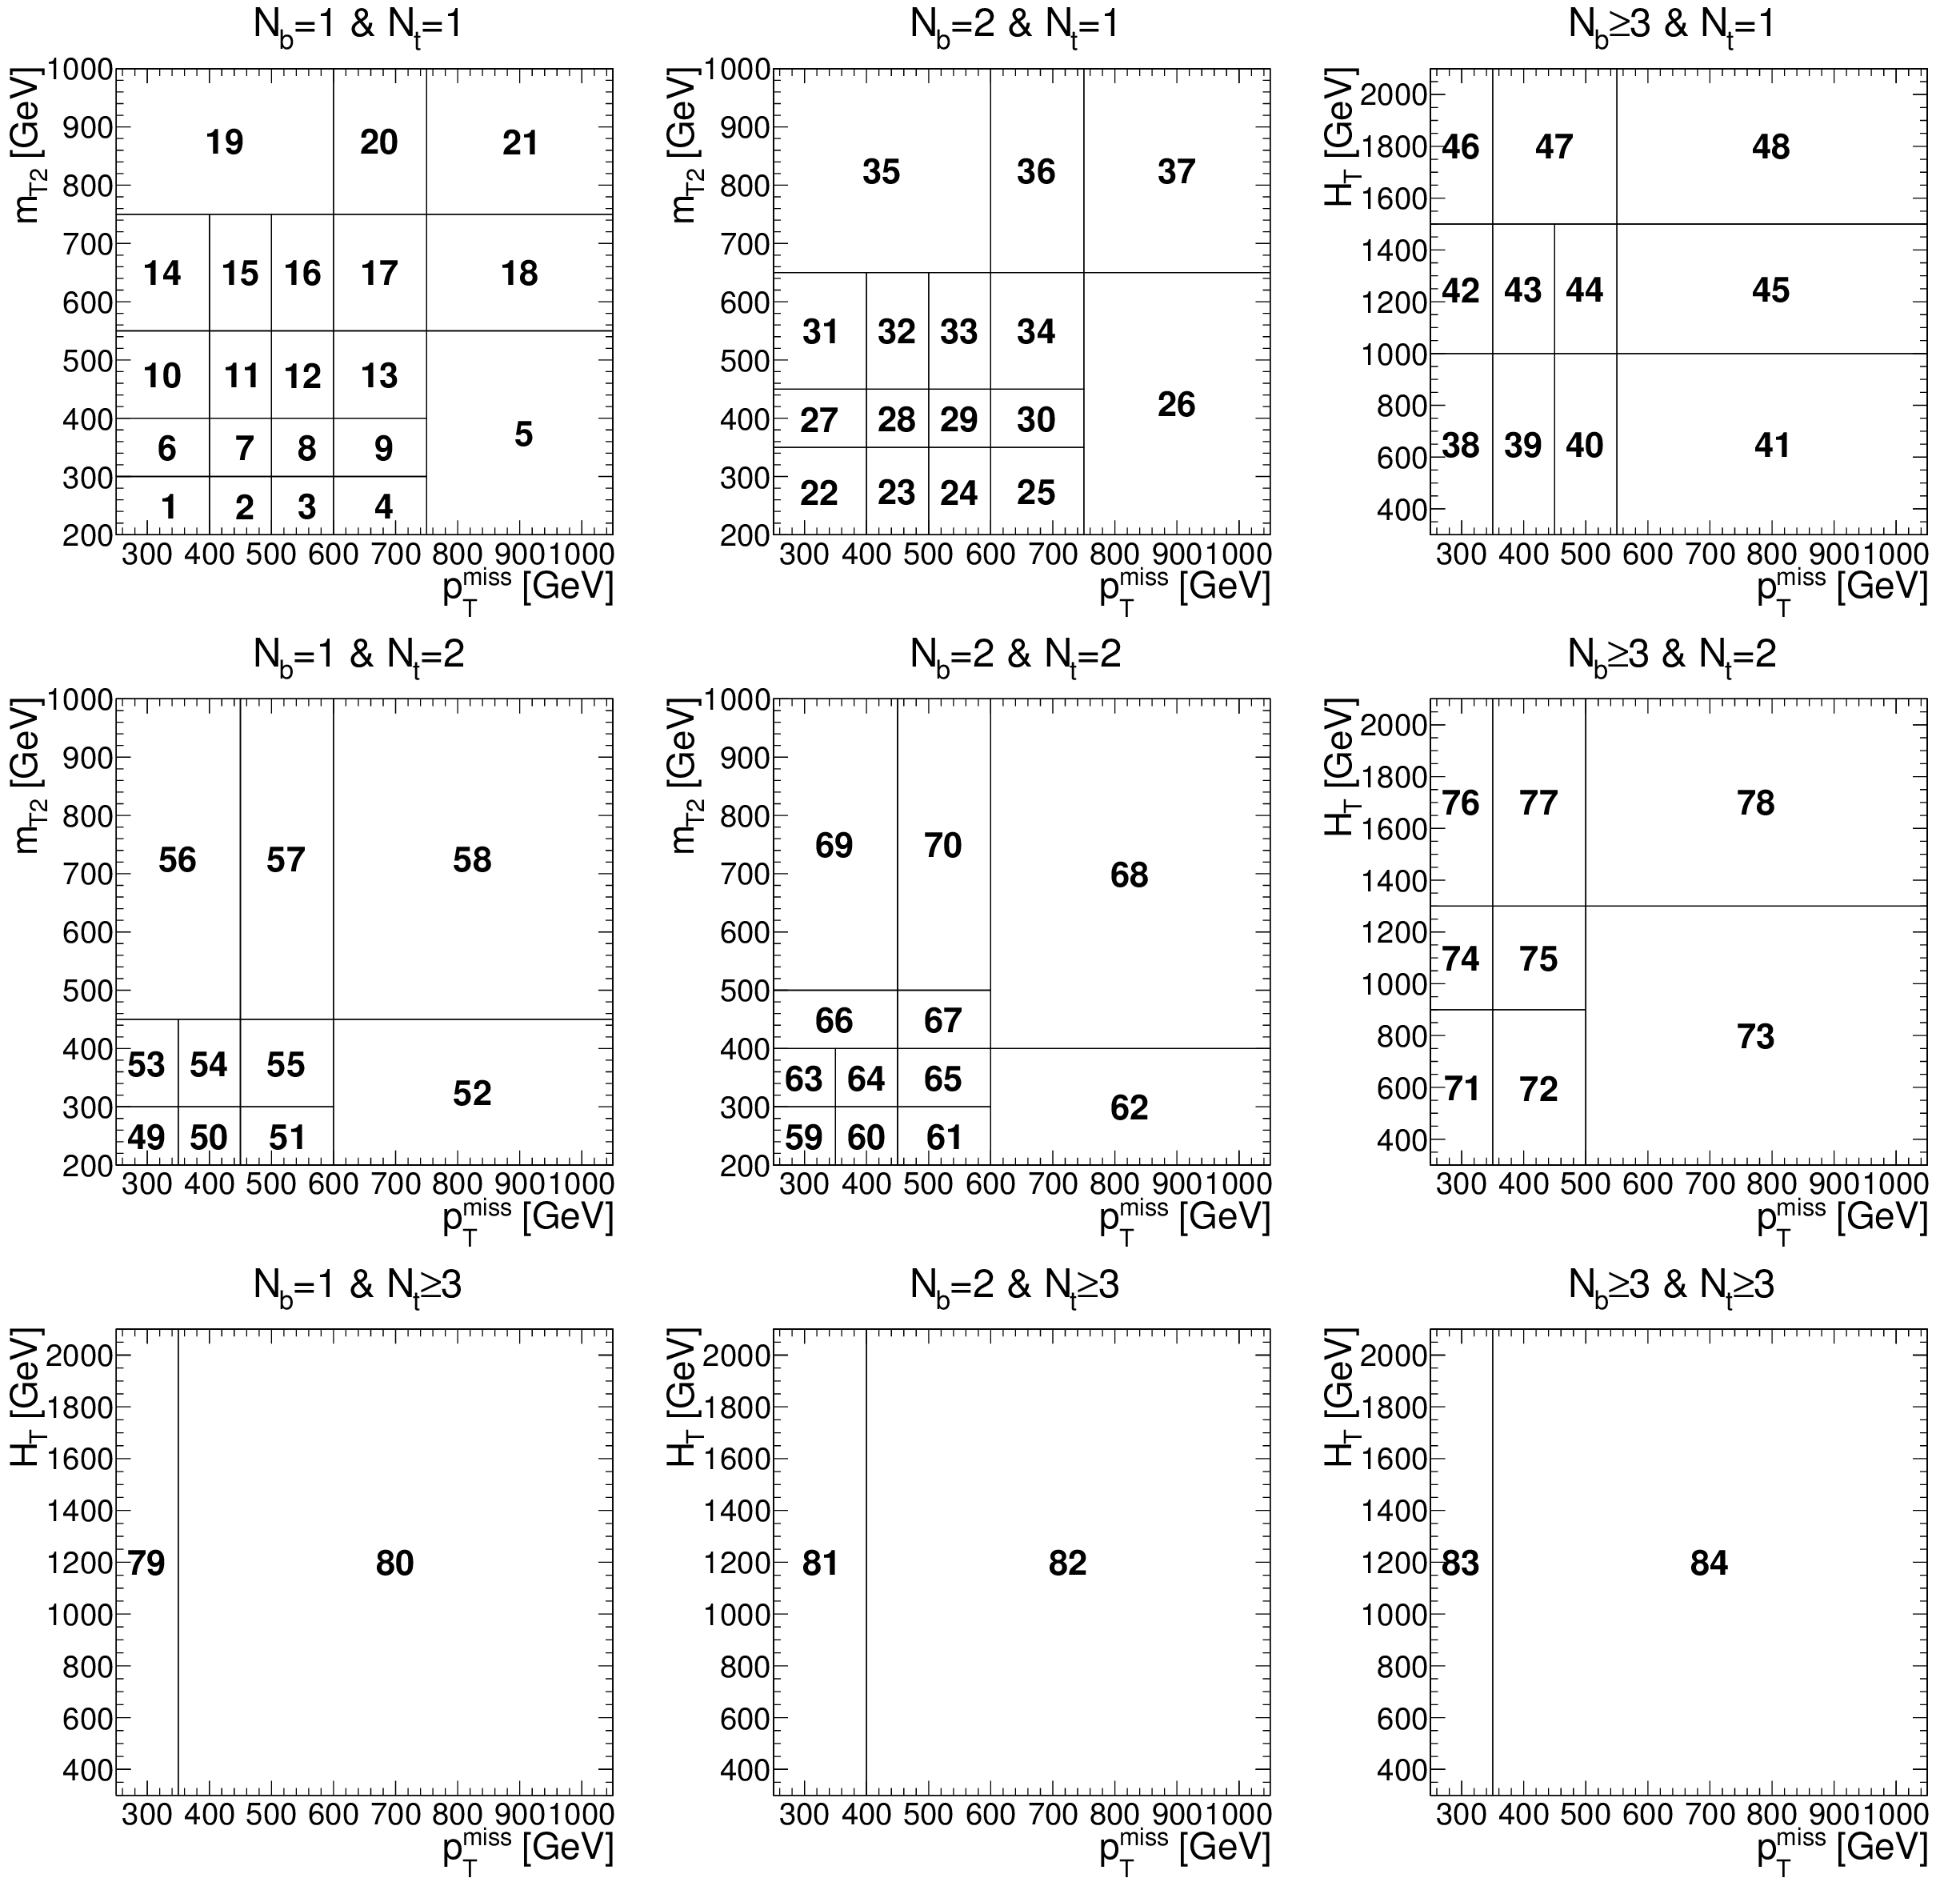
\includegraphics[width=0.9\textwidth]{SearchBins.png} 
\caption{Search region definitions in the kinematic variables.}
\label{SearchBins.png} 
\end{center}
\end{figure}

\section{Background Estimation}\label{backgrounds}

Since there are many SM processes which exhibit the same characteristics as those of the signal models (e.g. multiple jets, missing energy, etc.) it is of the utmost importance to be able to properly account for their contributions. These interactions, which closely resemble the signal that's being searched for, are called the SM background. However, they cannot be determined solely from the detector's reconstructed data itself, which is why MC simulation is used to recreate them using theoretical predictions from the SM. These simulations give us a good idea of what the signal region should look like if there were no signal events, and therefore any significant excess when comparing the MC background to data could signify a potential discovery. The relevant backgrounds for this particular analysis are: the lost-lepton background, the hadronic $\tau$ background, the Z $\rightarrow\nu \bar{\nu}$ background and the QCD multijet background.

\begin{figure}[tb]
\begin{center}
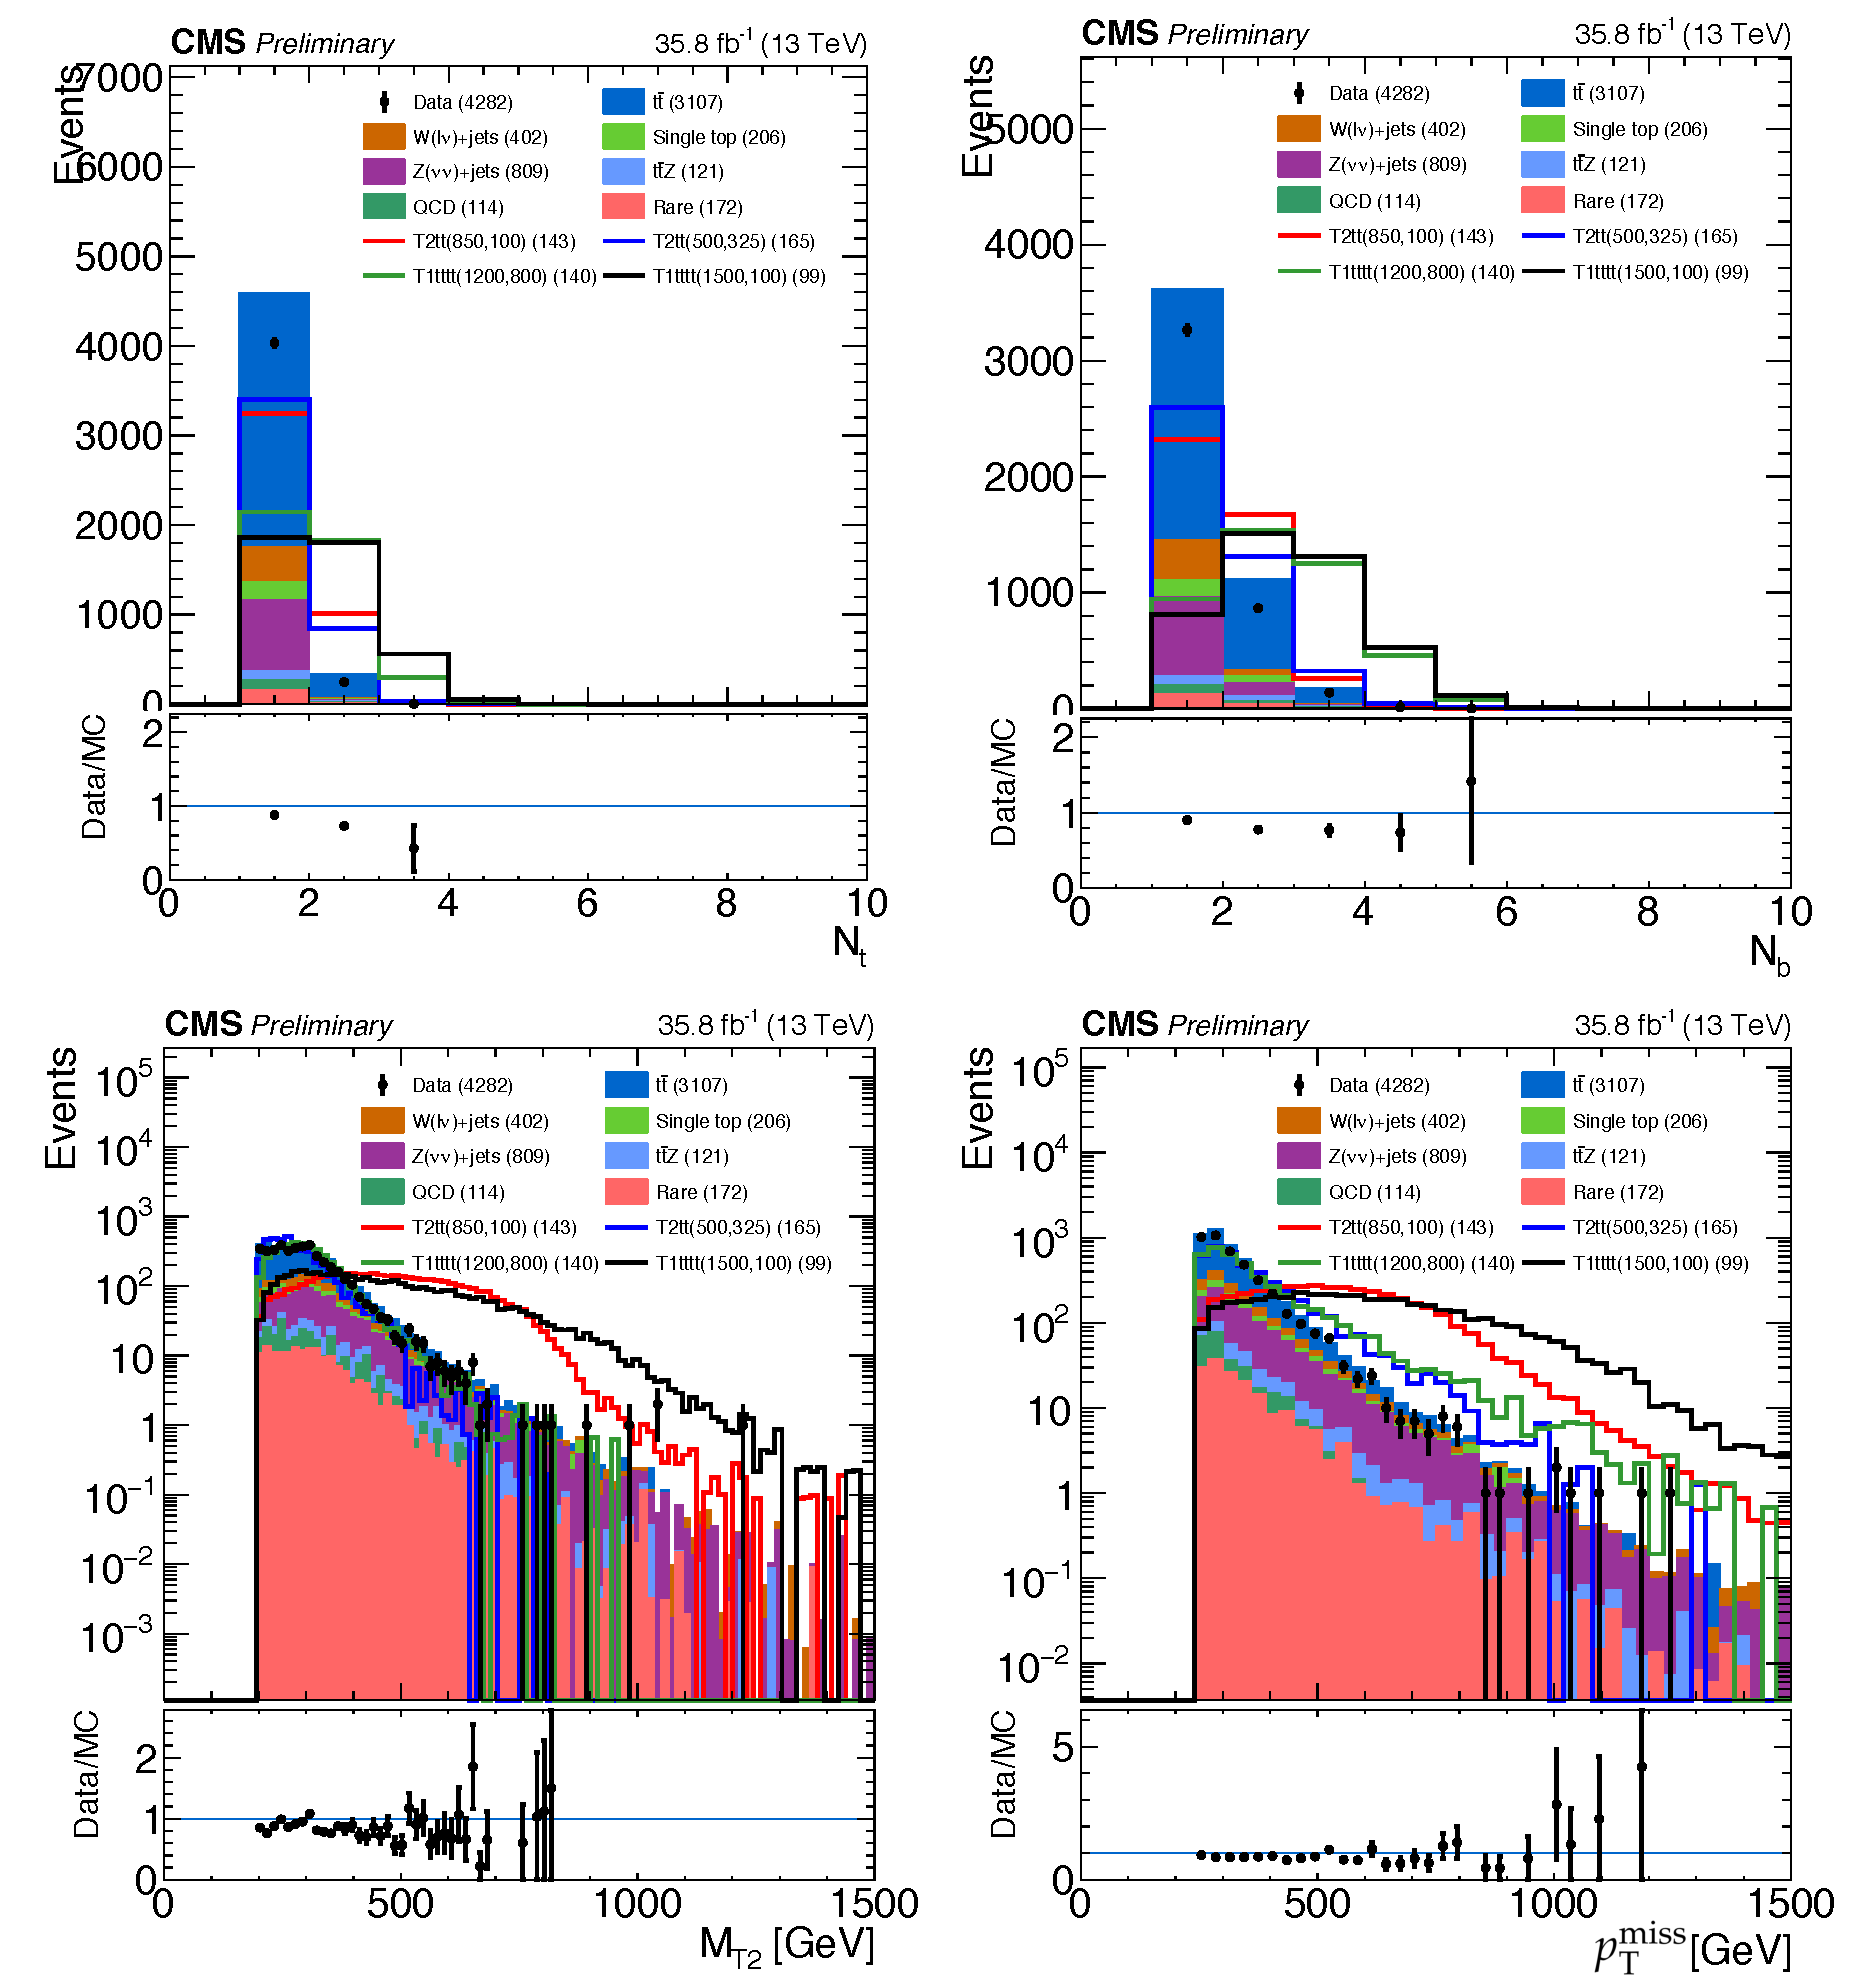
\includegraphics[width=0.9\textwidth]{MyPlots.pdf} 
\caption{Comparison between the total SM background from simulation and CMS data for $N_\text{t}$ (top left), $N_\text{b}$ (top right),  $m_\text{T2}$ (bottom left) and $p_{\text{T}}^{miss}$ (bottom right). Total SM backgrounds and signals are scaled to same data yield for a shape comparison.}
\label{MyPlots.pdf} 
\end{center}
\end{figure}

\subsection{Background from t$\bar{\text{t}}$, Single Top Quark and W+jets Events}

The vast majority of the expected SM background (around 70\%) is due to t$\bar{\text{t}}$ and W+jets events where the W decays into a lepton and a neutrino. Since the expected signal is purely hadronic, a portion of the leptonic and semi-leptonic decays are vetoed and do not form part of the total SM background. However, there are two different scenarios in which the lepton vetoes can be satisfied. For instance, when the W decays into a $\tau$ which decays hadronically ($\tau_\text{h}$), the $\tau$ gets reconstructed as a jet and passes the veto. If, on the other hand, the W decays into an electron or a muon, the veto is satisfied when the corresponding lepton is said to be ``lost". In other words, the lepton veto fails to reject events when light leptons (electrons and muons) are not isolated, not identified/reconstructed, or are out of the acceptance region. Both scenarios are evaluated together with a single-lepton data control sample (CS), subjected to the same trigger used for signal events.\\

The total predicted amount of lost-lepton and $\tau_\text{h}$ events in any given search region is defined by the net sum of single-electron and single-muon events in the respective CS, corrected by a translation factor that is determined from simulation. Due to differences in how they are detected, the single-electron and single-muon samples are determined separately. The translation factor used to correct the search bins is defined as the ratio of simulated $\tau_\text{h}$ and lost-lepton events in the search region over the number of simulated single-electron or single-muon events in the corresponding CS region.

\begin{figure}[H]
	\begin{center}
		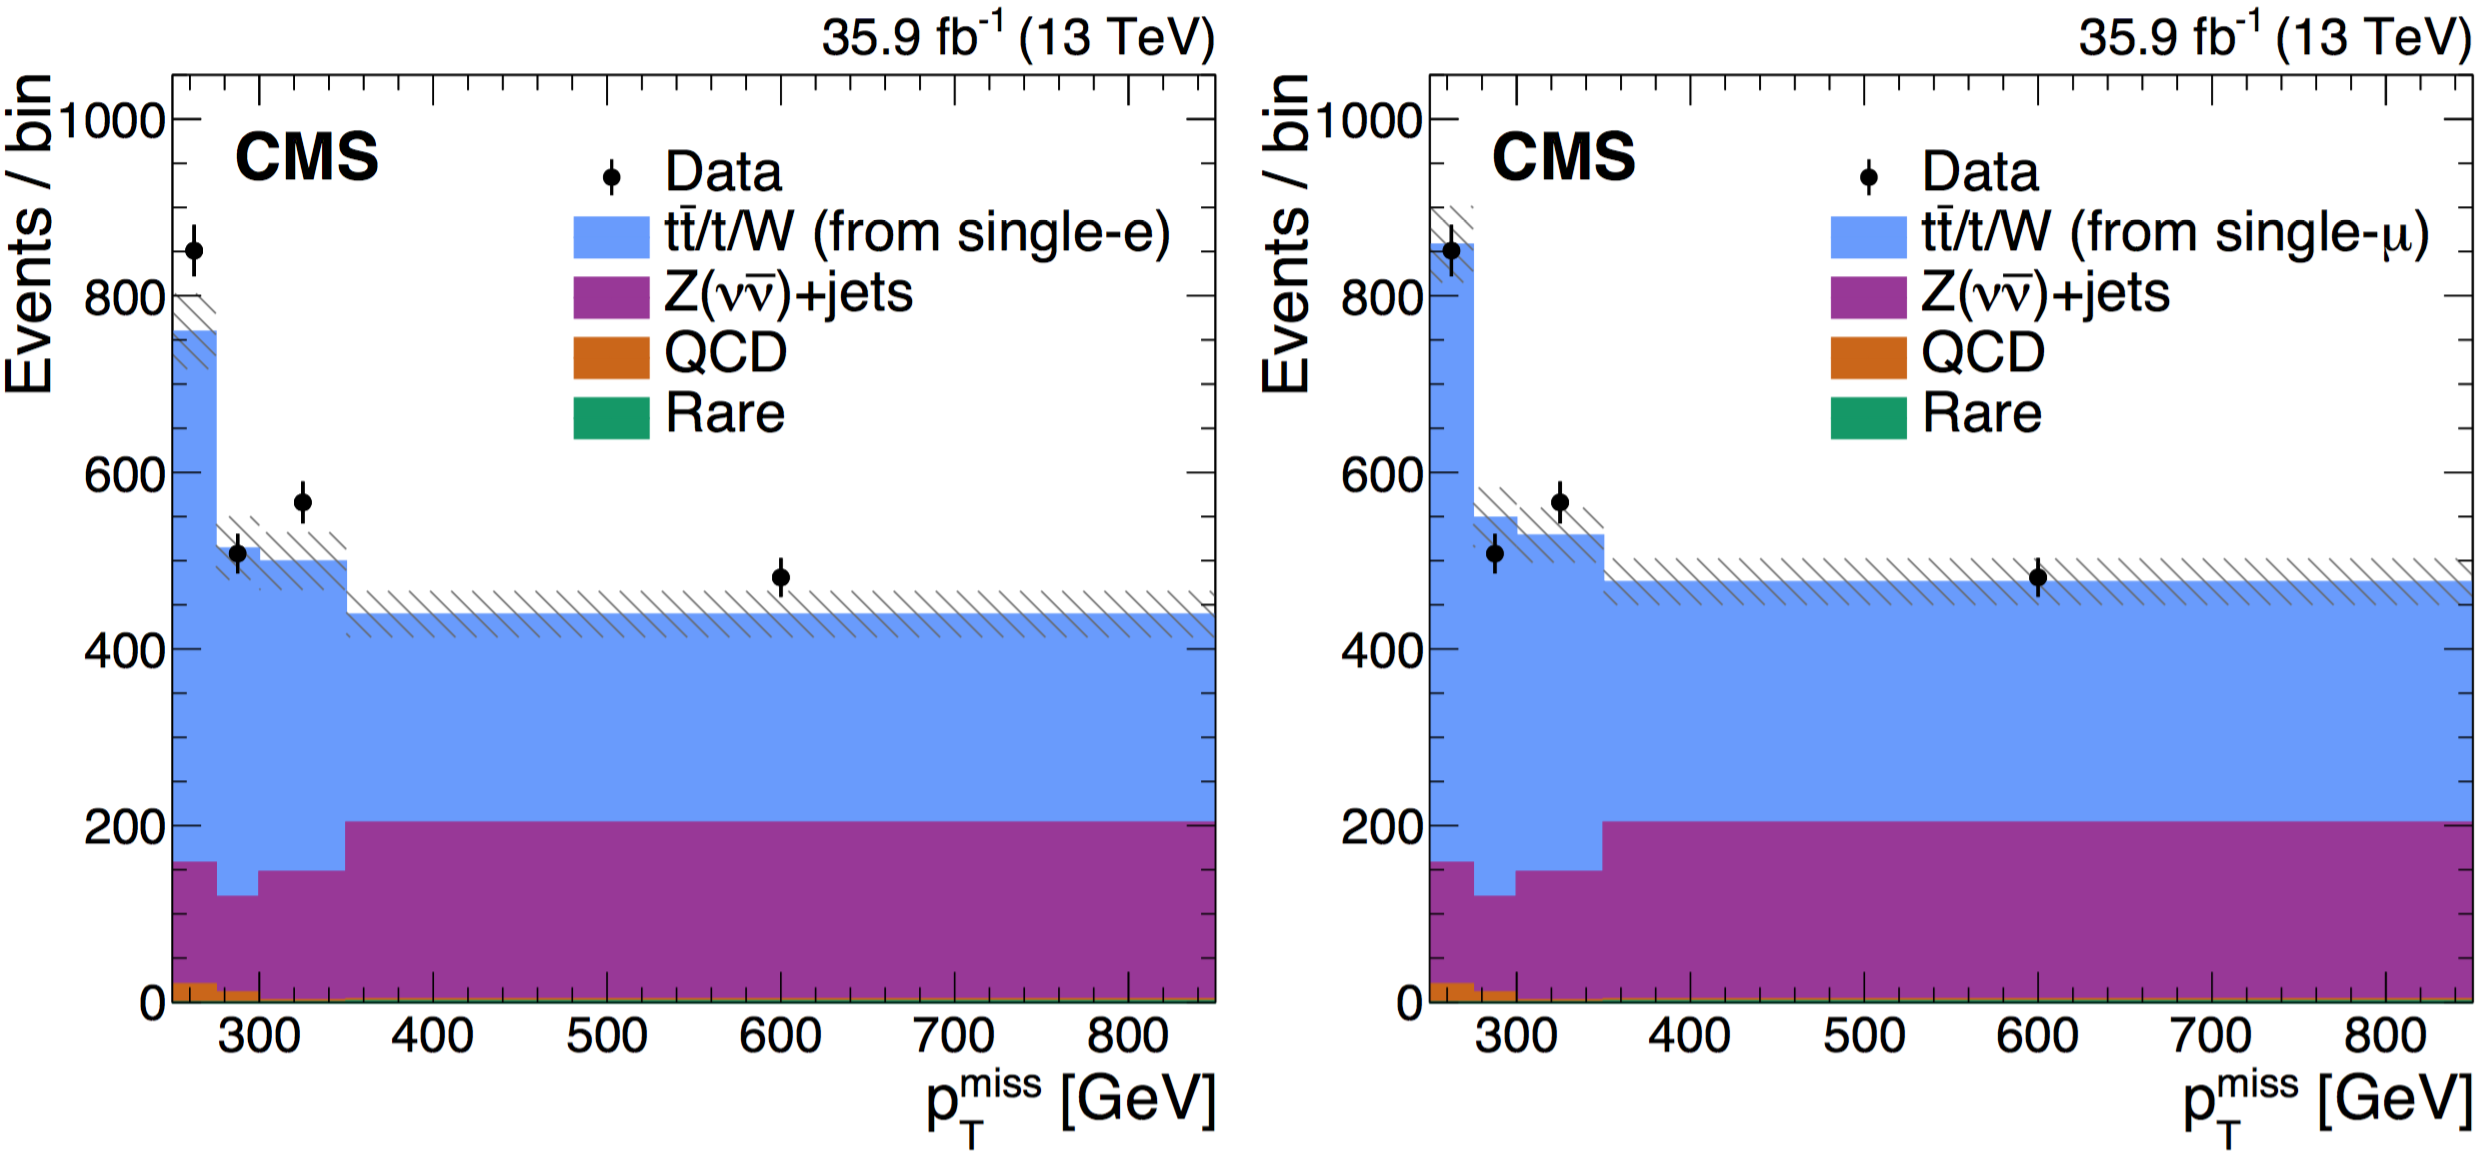
\includegraphics[width=0.8\textwidth]{LL.png} 
		\caption{Distribution of $p_{\text{T}}^{miss}$ for both the single-electron (left) and single-muon (right) SB data samples compared to predictions for SM processes. The hatched bands indicate the statistical uncertainties in the total SM prediction. Note that the data and the predictions for all backgrounds except that for t$\bar{\text{t}}$, single top quark, and W+jets events are identical between the left and right plots.}
		\label{LL} 
	\end{center}
\end{figure}

In order to test this method, a sideband (SB) region is selected which is orthogonal to the search region. This region is defined by the same selection criteria applied to data except for $N_t = 0$, $N_b \geq 2$, and $\Delta\phi$($p_{T}^{miss}$,  j$_\text{1,2,3,4}$)$~> 0.5$, where the last two requirements are applied in order to suppress contributions from Z($\nu\bar{\nu}$)+jets and QCD multijet processes. The SB is divided into four intervals of $p_{T}^{miss}$, where the contribution of lost-lepton and $\tau_\text{h}$ to the corresponding intervals are determined by multiplying the appropriate single -electron and single-muon CS (\autoref{LL}) by a translation factor from simulation. The contribution to the SB from other backgrounds, such as Z+jets, QCD multijet and rare events, is estimated directly from simulation. The total SM background prediction is found to agree with the data within uncertainty, confirming the validity of the translation factor procedure.\\

Systematic uncertainties stemming from the prediction of t$\bar{\text{t}}$, single top quark and W+jets background events are determined from various sources: The statistical uncertainty associated to the translation factors determined for each search region (1--40\%), the lepton reconstruction and isolation efficiency (7--43\%), the jet and $p_{\text{T}}^{miss}$ energy scale and resolution (maximum of 64\%), the ISR modeling (maximum of 13\%), the PDF's (maximum of 32\%) and the b-jet tagging efficiency (1\%).

\subsection{The Z $\rightarrow\nu\bar{\nu}$ Background}\label{ZnunuSection}

The Z $\rightarrow\nu\bar{\nu}$ background is derived using simulated Z $\rightarrow\nu\bar{\nu}$ events that have been corrected for observed differences between data and simulation. In order to correctly estimate this background two scale factors are used to weigh the simulated events: $R_{norm}$ and $S_{DY}( N_j)$  which correct the normalization of the simulation and the shape of the simulated $N_j$ distribution, respectively. These scale factors are calculated from the dimuon control region which includes events with two muons and no muon or isolated track veto. In the region where $81 < m < 101$ GeV, the two muons are treated as if they were neutrinos.\\

The first scale factor, $R_{norm}$, is computed by comparing the expected event yield in the dimuon control region from the Drell-Yan (DY) simulation with the observed event yield in data after subtraction of the other SM processes. The second scale factor, $S_{DY}$, depends on the number of jets ($N_j$) in the event and is also computed from the dimuon control region in which the signal region requirements on $p_\text{T}^{miss}$, $N_t$ and $m_\text{T2}$ are removed, and the $H_\text{T}$ requirement is relaxed to $H_\text{T} > 200$ GeV. For each $N_j$ bin this scale factor is calculated from the ratio between data and the DY simulation. Its value ranges between 0.6 and 1.1, depending on the $N_j$ bin.

\begin{figure}[H]
	\begin{center}
		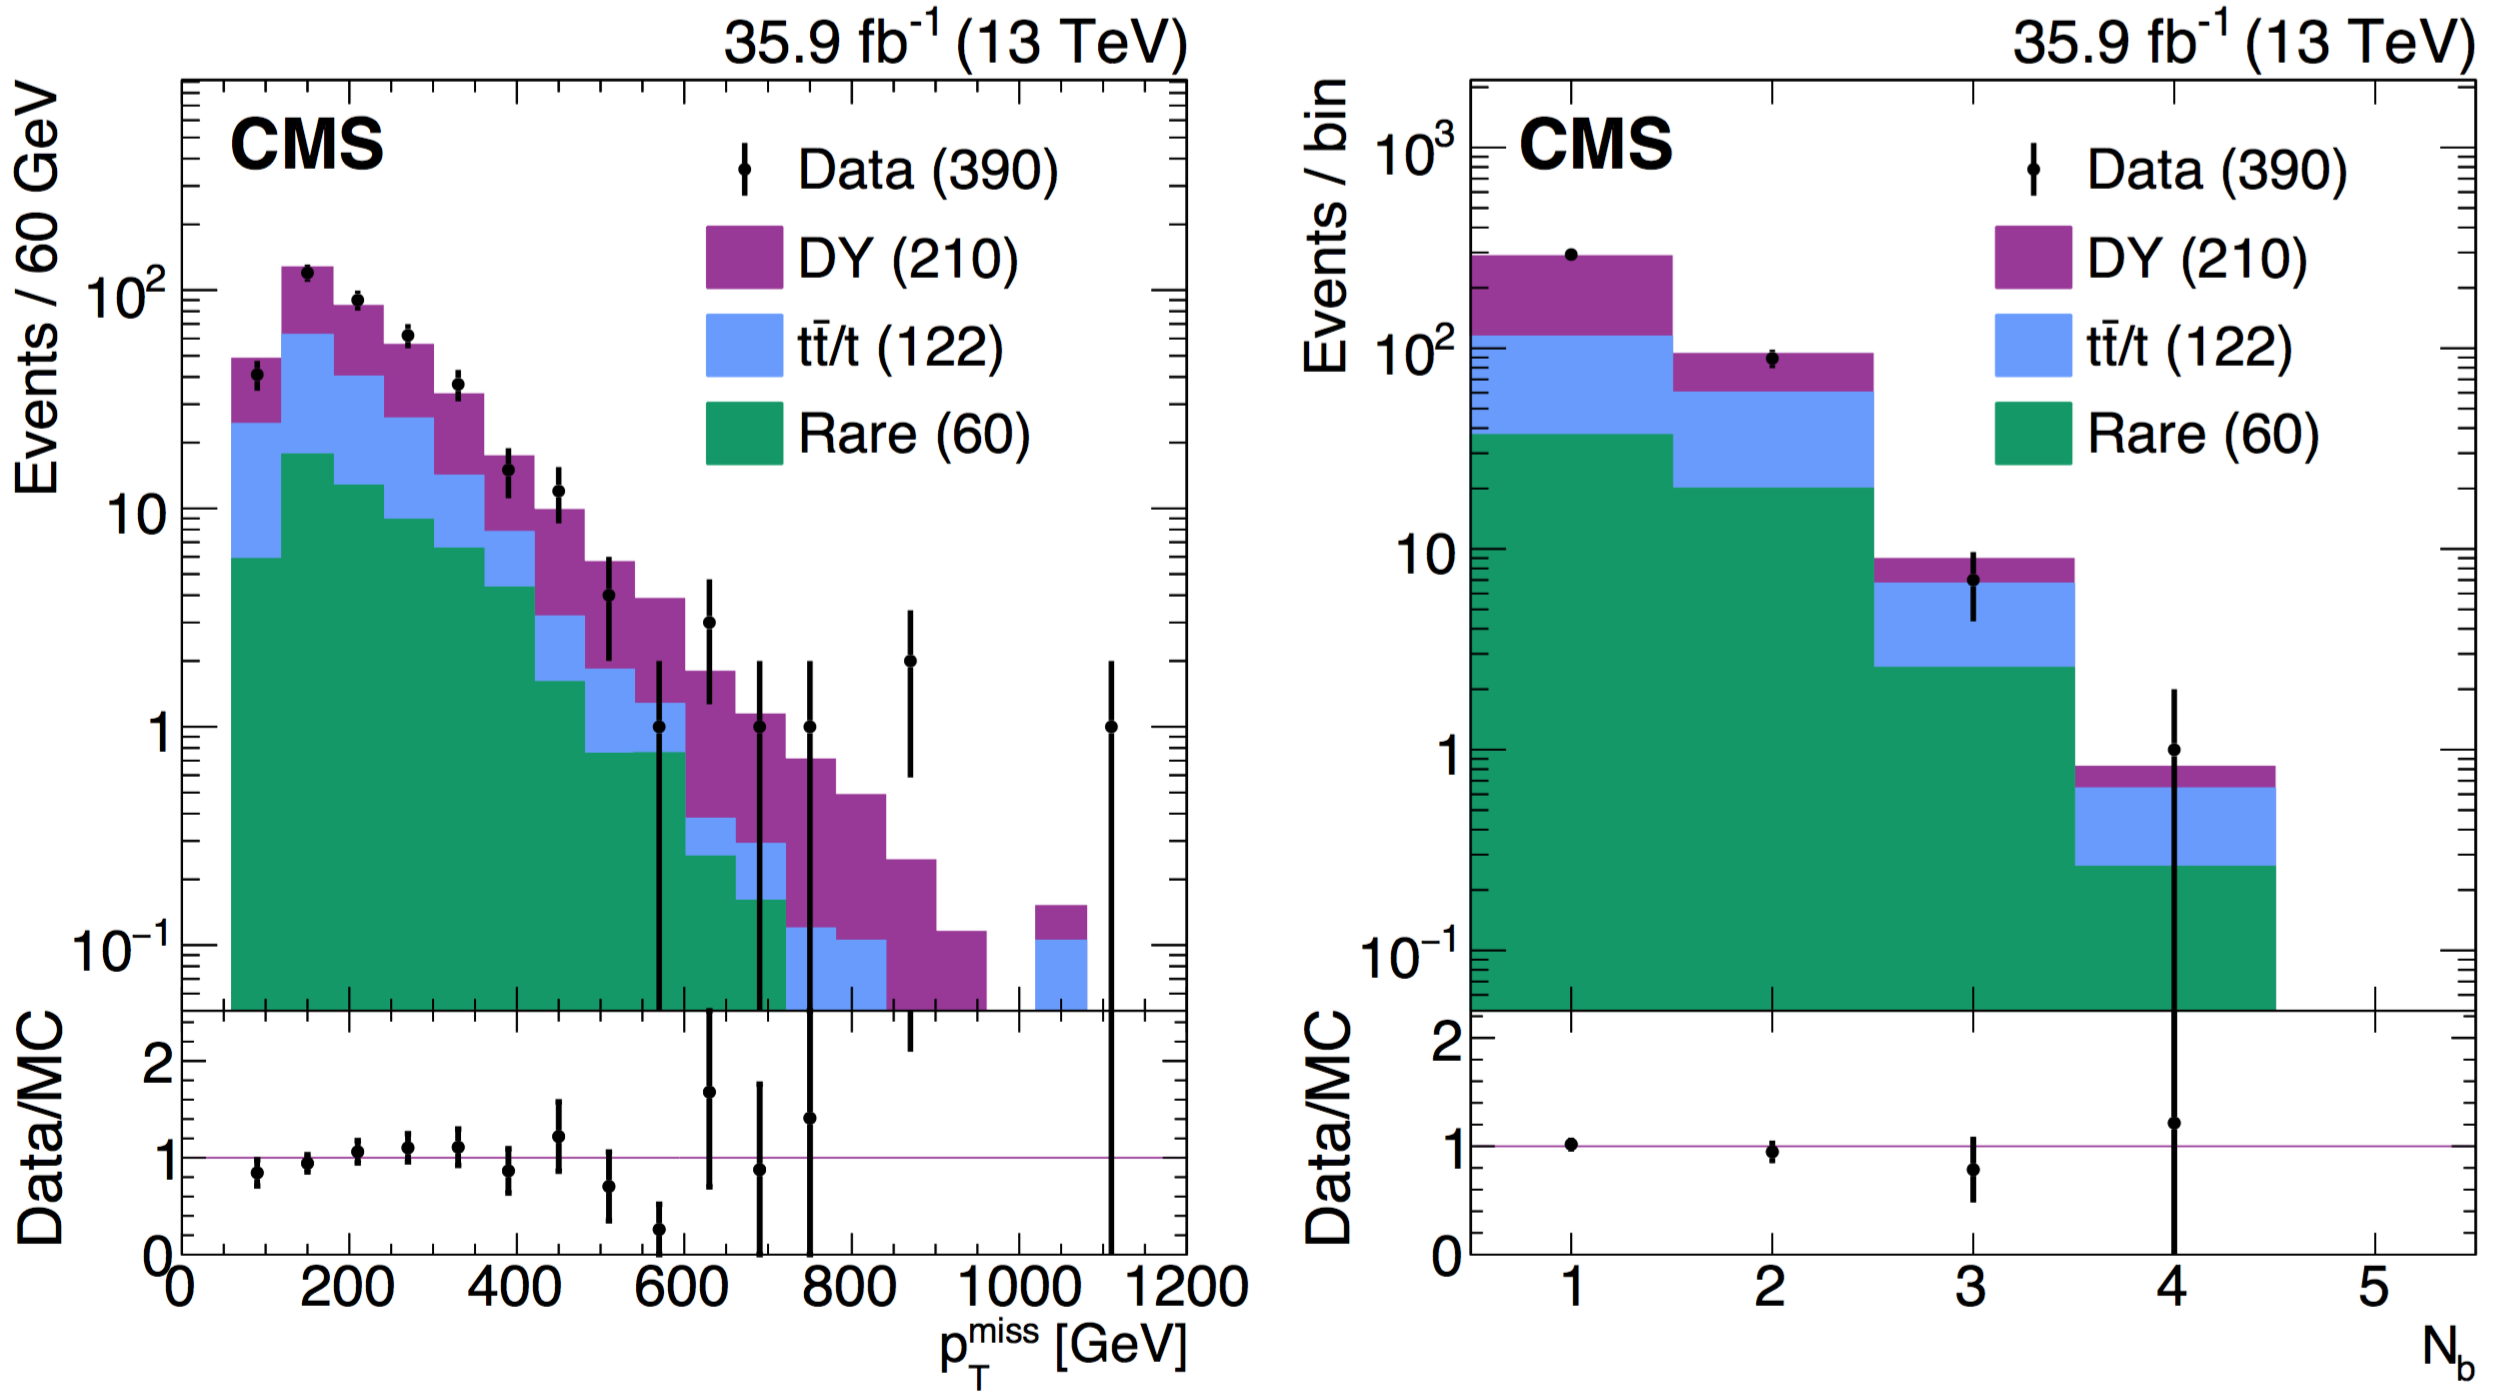
\includegraphics[width=0.8\textwidth]{Znunu.png} 
		\caption{The $p_\text{T}^{miss}$ (left) and $N_b$ (right) distributions of data and simulation in the loose dimuon CS after applying both the normalization and shape correction factors. The lower panels show the ratio between data and simulation. Error bars in the plot account only for statistical uncertainties. The values in parentheses indicate the integrated yields for each component.}
		\label{Znunu} 
	\end{center}
\end{figure}

The systematic uncertainties for the Z($\nu\bar{\nu}$)+jets background are obtained from the shape differences between data and simulation in the loose dimuon CS in terms of the $N_b$, $N_t$, $p_{\text{T}}^{miss}$, $m_\text{T2}$ and $H_\text{T}$ after the normalization factor ($R_{norm}$) has been applied. These include the statistical uncertainty in the $N_j$ shape correction (1--46\%) and in the overall normalization correction (7.6\%). Additional systematic uncertainties account for the jet and $p_{\text{T}}^{miss}$ energy scales (1--71\%), the b tagging efficiency (1--23\%), the PDFs and the renormalization and factorization scales (1--48\%), the statistical uncertainty in the simulation (1--81\%, with some search regions as high as 100\%), and the trigger (up to 14\%). An additional uncertainty is defined from the shift in the central value between the data and simulation in the distributions (14--44\% depending on the search region).

\subsection{The QCD Multijet Background}

To estimate the QCD Multijet background a signal-depleted, QCD multijet-rich data control sample is used. This control sample is defined by inverting the preselection requirements on $\Delta\phi$ ($p_\text{T}^{miss}$,  j$_\text{1,2,3}$) and subtracting contributions of other SM backgrounds, such as t$\bar{\text{t}}$, W+jets, and Z +jets. For t$\bar{\text{t}}$ and W+Jets the same methods (lost-lepton and hadronic $\tau$) are used to estimate the contributions for this QCD multijet-enriched control region. In the case of the Z $\rightarrow\nu \bar{\nu}$ background, simulation is used for its estimation due to its small number. Following that, a translation factor, partly determined by data and partly by simulation, is used to convert the number of QCD multijet events measured in the data control region into a QCD multijet prediction for each search region bin. This translation factor, called T$_\text{QCD}$,  is computed as the simulated ratio between the signal region and the inverted-$\Delta\phi$ control region, in bins of $p_\text{T}^{miss}$ and $m_\text{T2}$ where the bins are bounded in the same way as the signal bins.\\

The systematic uncertainty associated with the QCD multijet background for each search region is obtained as the difference between the event yield from simulation of QCD multijet processes and the prediction obtained by applying the background prediction procedure to simulated QCD multijet samples (30--500\%). Other sources include the statistical uncertainty in the translation factors (30--300\%) and the subtraction of the non-QCD-multijet SM contributions to the QCD control sample (2--50\%).

\subsection{Background From Rare and Other Processes}

The background contribution from rare processes forms only a tiny fraction of the overall SM background and has therefore a small effect on the final result. The estimation for these processes are determined directly from simulation, with the biggest contribution coming from t$\bar{\text{t}}$Z. With the exception of the t$\bar{\text{t}}$Z process, all other remaining backgrounds are combined. The comparison between simulation and the obtained data were found to be in agreement within a statistical uncertainty of 30\%, which is attributed to the systematic uncertainty in the estimation of the t$\bar{\text{t}}$Z background.

\section{Results and Interpretation}

\begin{figure}[H]
\begin{center}
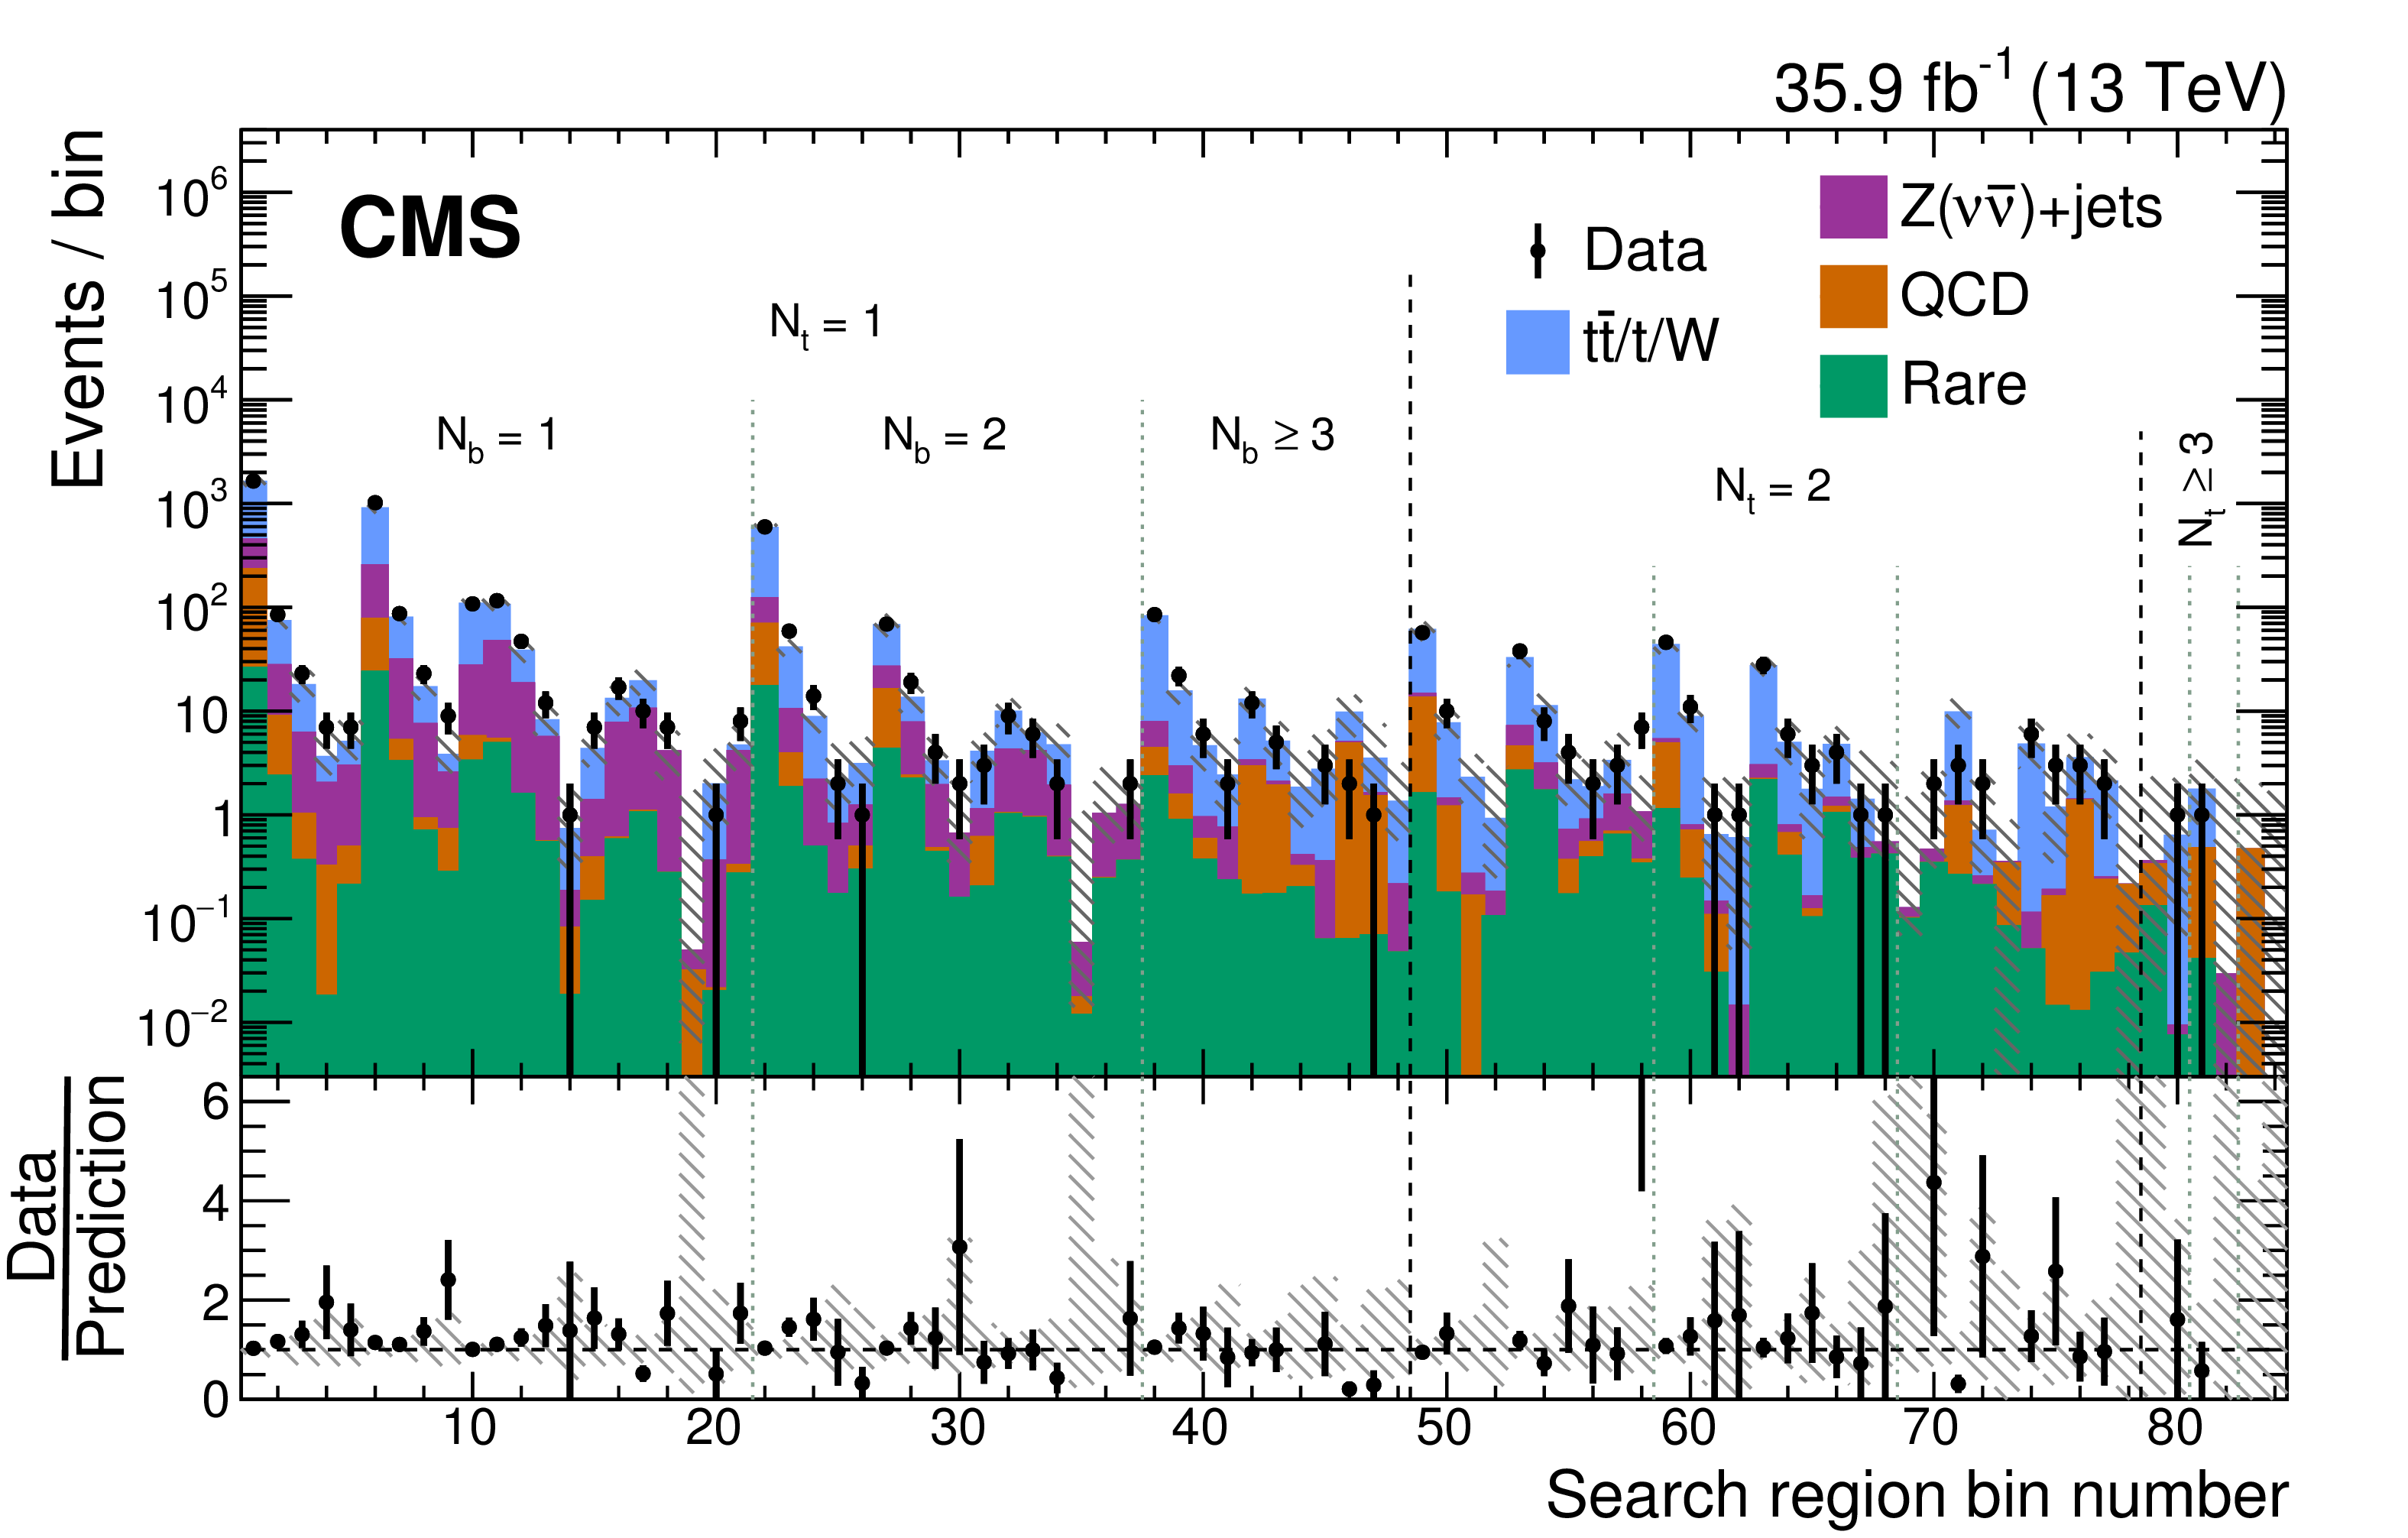
\includegraphics[width=0.8\textwidth]{SearchBinResults.png}  
\caption{Observed events compared to the corrected SM background predictions for all 84 search regions in the full data of 35.9 fb$^{-1}$ collected in 2016. The lower panel shows the ratio between the data and the total SM simulation. The gray bands show the total uncertainty related to the background prediction.}\label{SearchBinResults}
\end{center}
\end{figure}

\autoref{SearchBinResults} shows the summary of all observed events compared to the corrected SM background simulation for all of the 84 search bins. The data obtained shows no statistically significant deviation from the predicted SM background. The biggest contribution to the background is attributed to the t$\bar{\text{t}}$ and W+jets processes, followed by Z($\nu\bar{\nu}$)+jets, which could be dominant in regions that have a high $p_\text{T}$ threshold. The contributions arising from the QCD multijet and rare backgrounds are found to be nearly negligible in all of the search regions.\\

Exclusion limits are calculated for each of the signal models discussed in this chapter by applying a binned likelihood fit on the data. The likelihood function is obtained for each of the 84 search regions as well as for each of the background data control samples (single-electron, single-muon, and QCD) from the product of the Poisson probability density function. Exclusion limits were placed on the top squark, gluino and LSP production cross-sections with a 95\% confidence level (CL), calculated using a modified frequentist approach with the CL$_s$ criterion \cite{CL1,CL2} and asymptotic results for the test statistic\cite{stat1}.\\

\begin{figure}[H]
	\begin{center}
		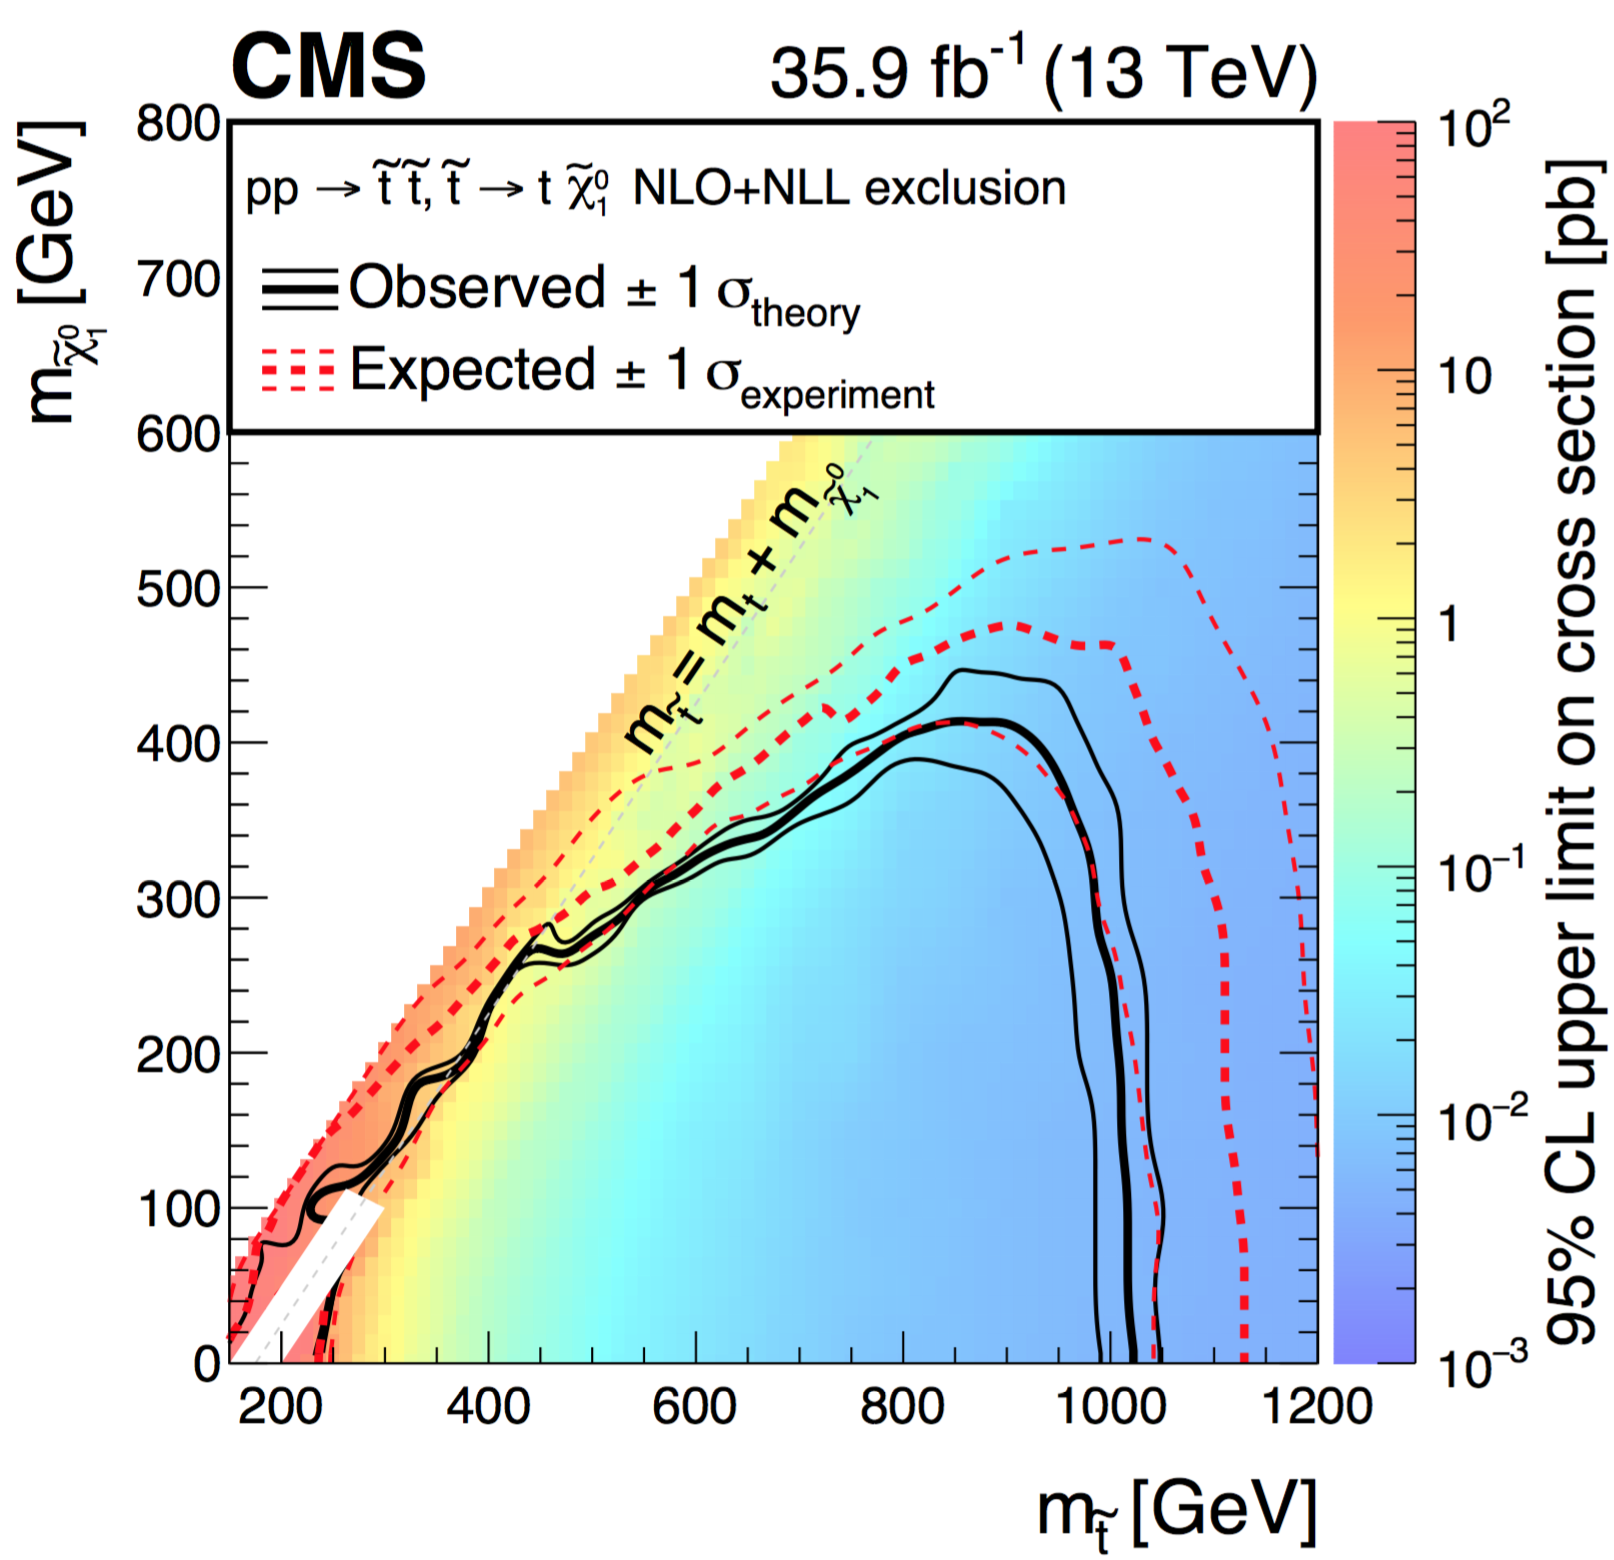
\includegraphics[width=0.55\textwidth]{T2ttLimit.png} 
		\caption{The 95\% CL upper limit on the production cross section of the T2tt simplified model as a function of the top squark and LSP masses. The solid black curves represent the observed exclusion contour with respect to NLO+NLL\cite{NLONLL} signal cross sections and the change in this contour due to variation of these cross sections within their theoretical uncertainties. The dashed
red curves indicate the mean expected exclusion contour and the region containing 68\% of the
distribution of expected exclusion limits under the background-only hypothesis.}\label{T2ttLimit}
	\end{center}
\end{figure}

The uncertainties from the search region modeling are taken into account for each of the 84 bins and arise from several different sources: the statistical uncertainty in the simulated event samples, the integrated luminosity (2.5\%\cite{Lumi}), the lepton and isolated-track veto efficiencies (up to 6.8\%), the b tagging efficiency (up to 21\%), the trigger efficiency (up to 2.6\%), the renormalization and factorization scales (up to 3.5\%), the ISR modeling (up to 46\%), the jet energy scale corrections (up to 34\%), the top quark reconstruction efficiency (up to 14\%), and the modeling of the fast simulation compared with the full simulation for top quark reconstruction and mis-tagging (up to 24\%). All of the uncertainties, with the exception of the statistical precision of the simulation, are taken to be fully correlated between the search regions. Contributions from signal contamination in the signal modeling are found to be only significant from the single-lepton control samples and negligible for the rest.\\

The 95\% CL exclusion limits obtained for the T2tt model (\autoref{T2ttLimit}), which consists of direct top squark production, excludes top squark masses up to 1020 GeV and LSP masses up to 430 GeV. Meanwhile, \autoref{Limits} shows the results for the gluino pair production models: T1tttt, T1ttbb, T5tttt, and T5ttcc. For the T1tttt model, gluino masses of up to 2040 GeV and LSP masses up to 1150 GeV are excluded, with corresponding limits of 2020 and 1150 GeV for the T1ttbb model, 2020 and 1150 GeV for the T5tttt model, and 1810 and 1100 GeV for the T5ttcc model. 

\begin{figure}[tb]
	\begin{center}
		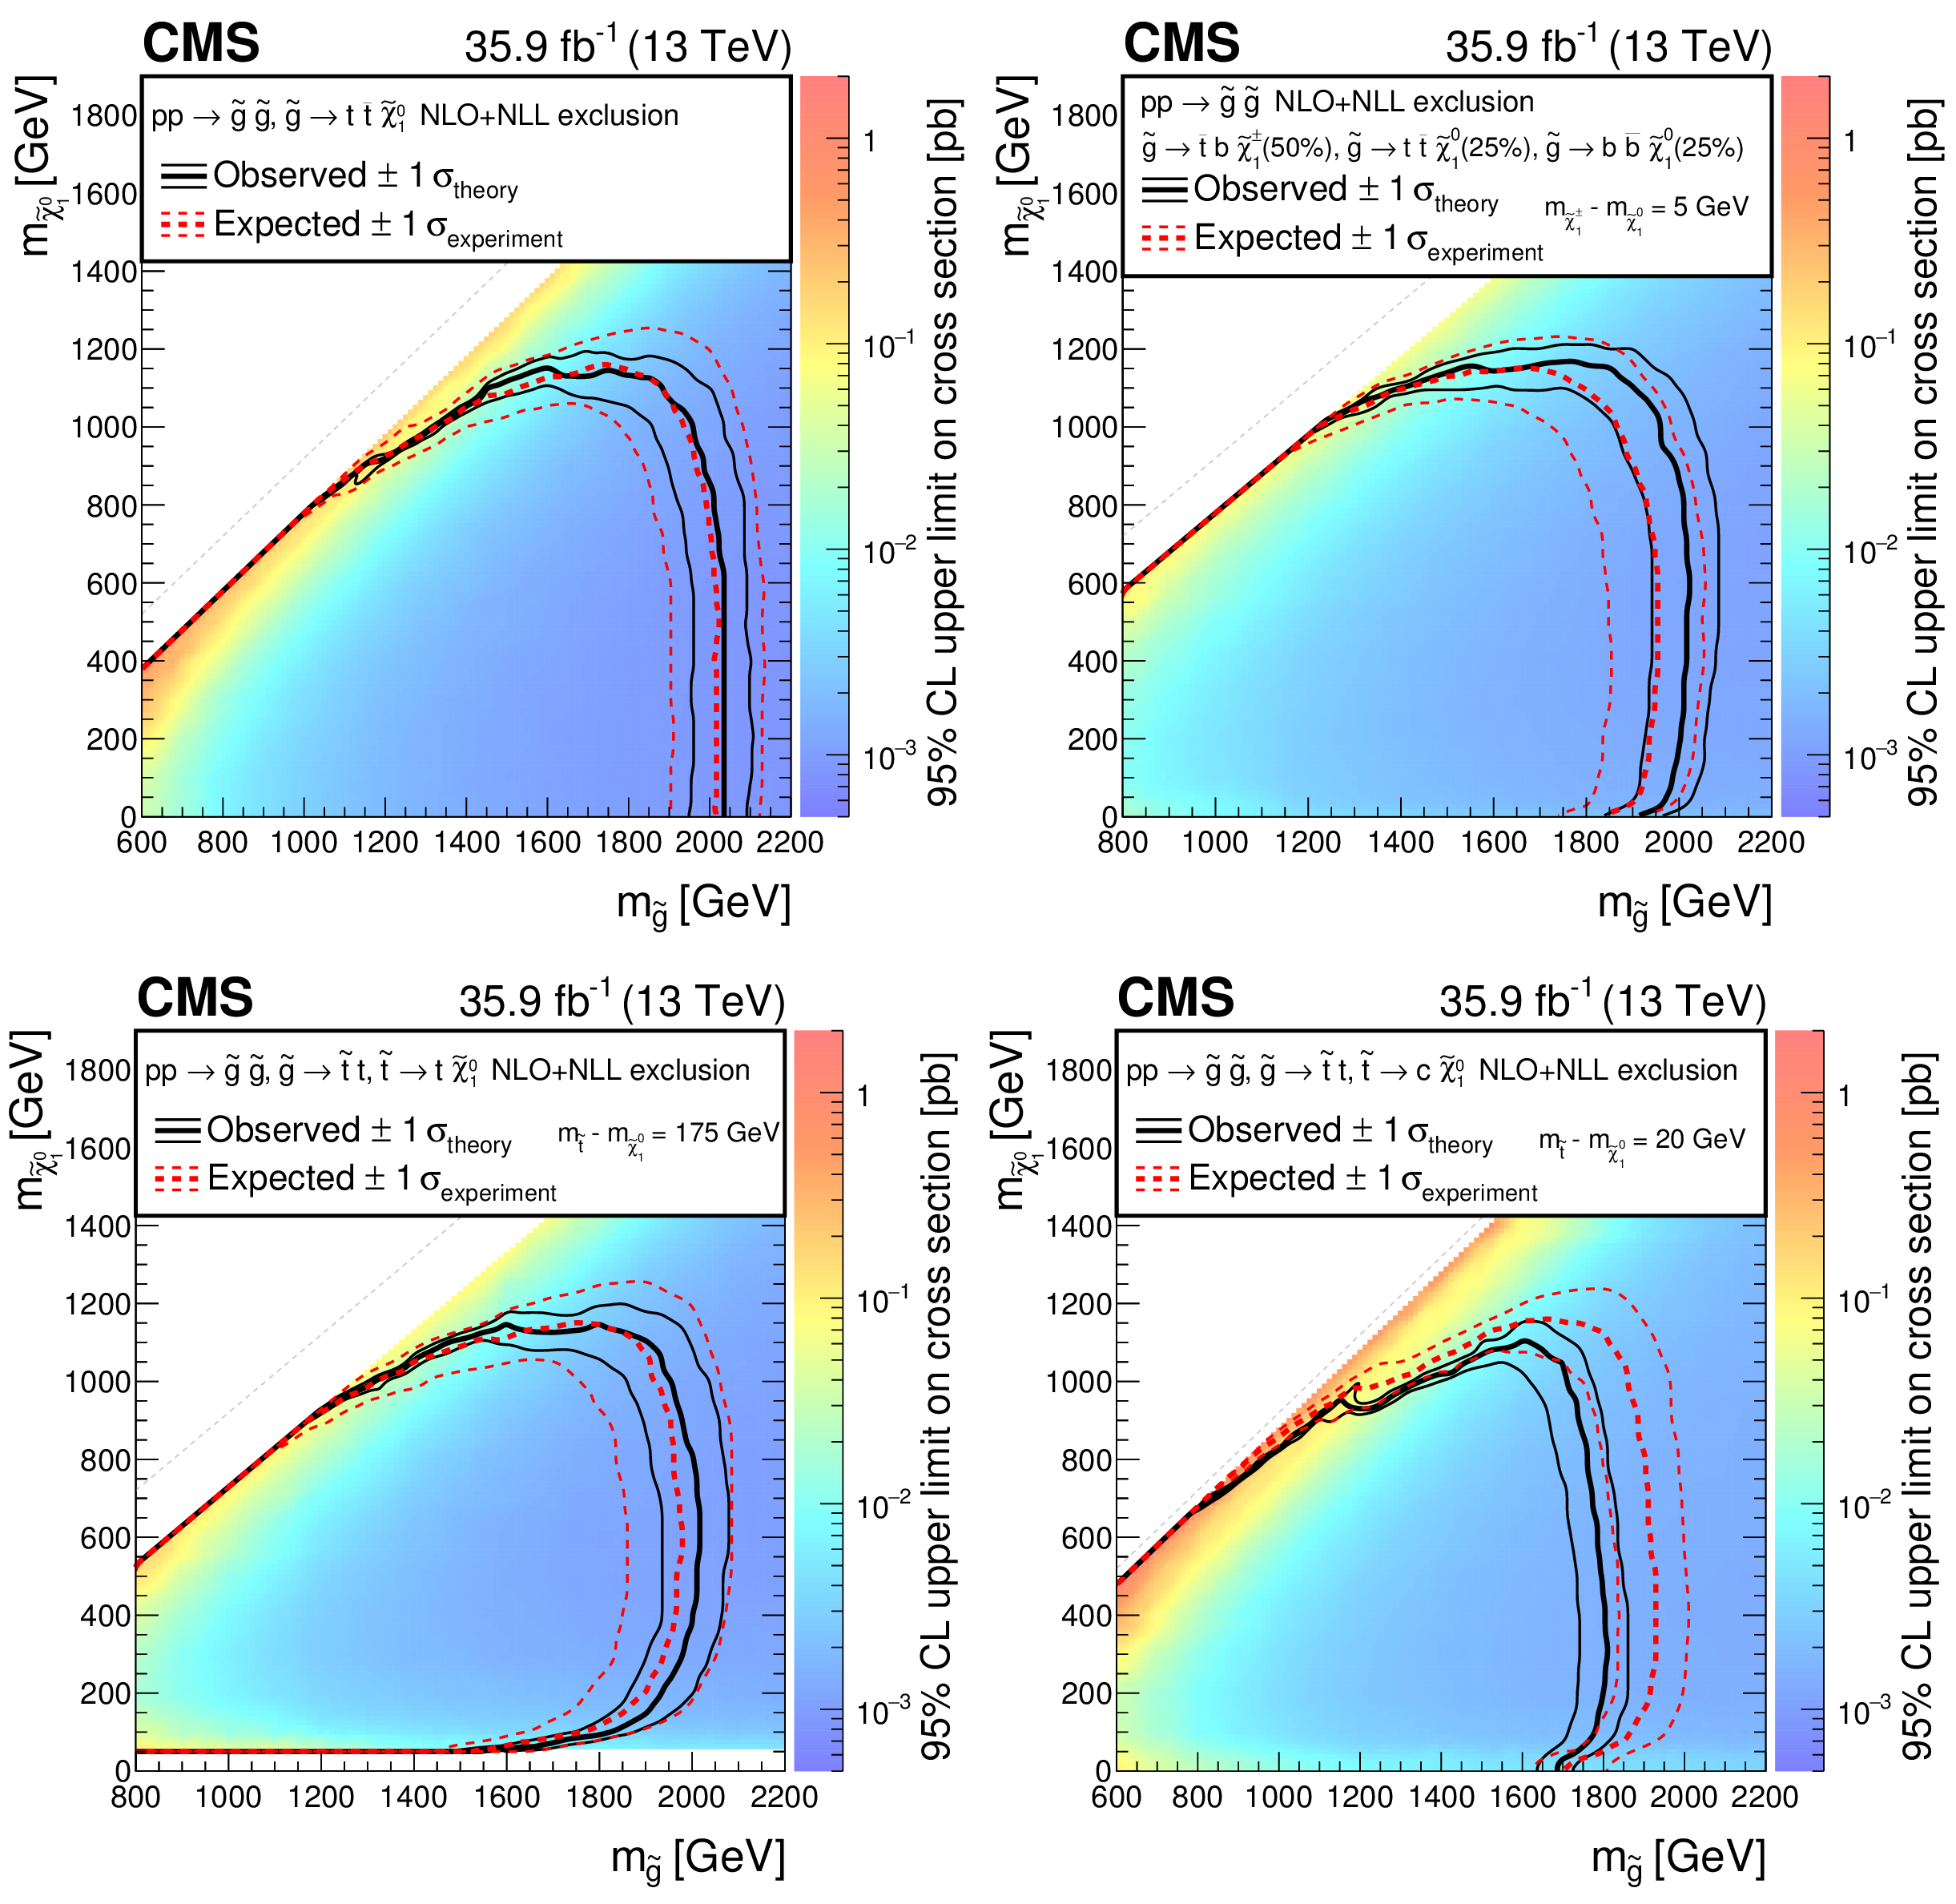
\includegraphics[width=1.0\textwidth]{Limits.png}
		\caption{The 95\% CL upper limit on the production cross section of the T1tttt (upper left), T1ttbb (upper right), T5tttt (bottom left), and T5ttcc (bottom right) simplified models as a function of the gluino and LSP masses.}\label{Limits} 
	\end{center}
\end{figure}

